% 2026-10-08 (interactive session, Claude Opus 5.5, per Leon: "provide a link to
%   the transport papers in the disclaimer ... for all v2.0 papers"). The
%   Authorship and disclosure paragraph now ends with one sentence giving the
%   Transport Papers community on Zenodo, as G01 gives it: "The papers of the
%   series are deposited in the Transport Papers community on Zenodo, \url{...}."
%   No other change; printed version stays 2.0. Recompiled: 28pp (unchanged), 0 errors,
%   0 overfull (unchanged), no undefined references. Script not re-run (no
%   computational content touched).
% v2.0 (2026-10-07, derivation session, Claude Opus 5.5, per rule 20, at Leon's
%   request: knock-ons of T12 v2.0 (Sections 10-11: the Pati-Salam route, the weak
%   angle, the grade-three direction w4(B - L), the registered 2-3 mixing route).
%   Printed version 1.0 -> 2.0 (\date), per Leon. No result renumbered; one label
%   appended (fact:gradethree, Fact 8.6, at the end of sec:weights after
%   fact:decomp, so no number moves). verify_T13.py unchanged.
%   sec:weights opening: "the one direction that carries the second family's
%   factor" -> "... on a single family, records the grade-three direction that
%   can carry it between families". cor:order: "available ... and only there"
%   now scoped to one-family mass forms, with a sentence on the second source
%   (Prop 8.1(iii)'s one-sided weighting, antisymmetric, giving entries between
%   families through an antisymmetric family coupling) and one on the route T12
%   registers (factor through 2-3 mixing; the pair-number requirement stands).
%   Proof cites the new Fact. NEW fact:gradethree (imported: T12 Prop 11.6, Obs
%   11.7, Rem 11.8). Levels (imported list), successor problem (6) (the 2-3
%   coupling, T12 successor problem (8)) and Position (both directions) updated.
%   Run: verify_T13.py 73/73 PASS (script unchanged), cloud workspace.
%   Compile: pdflatex x3, 28 pages (27 before), 0 errors, 0 undefined refs, 0
%   multiply defined, 0 overfull. Em dashes: 0.
%   Cross-references (rule 21): verify_crossrefs.py T13 67/67 both directions;
%   suite sweep 740 locators, 738 ok; the two failures are pre-existing and outside
%   this pass (T14a line 670, \cite[Premise P2]{ButlerT14}).
% T13 of the Transport Papers series.
% Correction (2026-09-10, mechanical pass, per Leon): rule 23 misidentified T5 as the printed-version exception. T1 is the exception at Version 3.0; every other paper, T5 included, reads Version 1.0. \date corrected accordingly (was 1.1).
% v1.1 (2026-09-10, derivation session, Fable 5.1 subagent, per rule 20,
%   series-review repair pass against series_review_2026-09-09.md).
%   Printed version 1.0 -> 1.1 in \date.
%   2.8: mass data refreshed to PDG 2024 (S. Navas et al. 2024), replacing
%     the PDG 2022 values that were cited as 2024. Inputs: m_e = 0.51099895
%     and m_mu = 105.6583755 now at full PDG precision (were 0.5110, 105.658;
%     the rounding of m_mu alone moved the deviation from 2/3 by 0.5e-6
%     relative, which is now the leading digit), m_tau = 1776.93 +/- 0.09
%     (was 1776.86 +/- 0.12), m_s = 93.5 (was 93.4), m_d = 4.70 (unchanged).
%     Every downstream figure recomputed in exact rational arithmetic
%     (Fraction, isqrt brackets, the script's own method), old -> new:
%     Sec 5 (prop:linearkill, Rem withdrawn, prop:nullity, Fig lightcone),
%     Sec 1, Obs 7.2 (obs:instrument), Sec 9 Part C:
%       Q_m 0.89356 -> 0.89357 (cos^2 theta_m, theta_m = 52.35 unchanged);
%       Q_sqrt(m) 0.6666608 -> 0.6666645; 2/3 - Q: 5.8e-6 -> 2.2e-6 absolute
%       ("six parts in 10^6" -> "two"), 8.8e-6 -> 3.3e-6 relative ("nine"
%       -> "three", at three sites incl. Fig caption and Sec 1);
%       predicted m_tau 1776.96 -> 1776.97 (bracket (1776.9, 1777.0) kept),
%       "one standard deviation" -> "half a standard deviation" (0.43 sigma);
%       s^2 : |d|^2 = 941.52 : 941.51 -> 941.55 : 941.55, equality 1.8e-5
%       -> 6.6e-6 ("two parts in 10^5" -> "seven parts in 10^6");
%       q(v) 0.017 -> 0.0062, |v|^2 = 1883 unchanged (1883.099 exact);
%       |Gamma|/a = 1.4142, delta = 0.222, x*, K/6, Cabibbo sqrt(m_d/m_s)
%       = 0.224 all unchanged at the printed digits (Prop ordered(2) proof:
%       0.2243 -> 0.2242, 0.3 -> 0.4 percent);
%       Obs 7.2 offset 4.4e-6 -> 1.7e-6 rad (exact 1.65e-6), resolution from
%       +/- 0.12 -> +/- 0.09 MeV: 5e-6 -> 3.8e-6 rad; the closing clause
%       now says the offset is below the resolution (was "same order").
%     Sec 9 Part C brackets restated to match the script (below).
%   2.5: bibitem ButlerT15 subtitle corrected to "The Empty Twistor, the
%     Seesaw Scale, and the Bet at the Floor". Other ButlerTn titles checked
%     against the brief's list, all exact. "refreshed at submission" in the
%     levels section is consistent with this refresh and left as is.
%   Script: verify_T13.py 73/73 (one mass table ME, MU, MT, MT_ERR at PDG
%     2024, also feeding the Part G RECORD lines, which previously used a
%     second rounded table; brackets retuned to the new central values:
%     d(theta) (4.3, 4.5)e-6 -> (1.6, 1.7)e-6, resolution (4.9, 5.2)e-6 ->
%     (3.7, 3.9)e-6, split (941.50, 941.53) -> (941.54, 941.56) with relative
%     difference < 1e-5 (was 2e-5), C(v) = 1883.09937445 exact; the 2/3 +/-
%     1e-5, Q_m, cos^2 theta_m, tan^2 delta, nullity and m_tau brackets
%     pass unchanged; labels reworded to the new figures; no check added).
%   Compile: pdflatex x2, 27 pages, 0 errors, 0 undefined refs, 0 multiply
%     defined, 0 overfull, no float overflow.
% PRINTED VERSION 1.3 (2026-09-08), review-repair pass; 1.2 and earlier blocks are history.
% v1.7 (2026-09-08, derivation session, Fable 5.1 subagent, per rule 20,
%   review-repair pass against T13_review_v6.md).
%   B1: new Fact 8.5 (fact:decomp) at the end of Section 8 after Rem 8.4:
%     16 x 16 = 10 + 120 + 126 with the grade dictionary, 126bar acting as
%     zero on the 16, Provenance Slansky 1981; Prop 8.1(i) restated: pure
%     grade five, hence no 10 and no 120 component, and the induced mass form
%     on the 16 is the 126 component (Spin(10)-equivariance, in the proof).
%   B2: (S) named in Prop 8.1(ii), (iv) and Cor 8.3; the levels' (S)
%     paragraph runs Sections 5 to 8 and names the Clebsch readings; the
%     Proved entry for Prop 8.1 is qualified; species table cited to T12
%     Prop 5.8 (S2). B3: Prop 7.5 states its premise (m/M_P invariant with m
%     fixed, the observation-level reading of T12 Prop 7.6(1)) with its
%     level; its levels entry moved from Proved to the imported paragraph.
%   S1: identity now w_4 chi = w_4(1 - 2 n_5). S3: Cor 8.3 and the Section 8
%     preamble use T17 Table 4 row 10's current order. S4: T12 Prop 9.32 for
%     uniqueness. S5: 120 + 126 to T12 Prop 9.15(b). S6: (iv) a magnitude,
%     signs recorded. S7/N1: Section 10 entries -1 and +-1/3. S8: y_e, y_d
%     scoped. S9: family no-go, up-type and Part G second check rebuilt (see
%     verify_T13.py docstring). S10/N19: Prop 7.5's proof describes the
%     script. S11: Cor 8.3 under Proved with its (S) condition and imports.
%   Also N2, N4 (Prop 7.5 title: kinematic), N5, N6, N7, N9, N12 (four
%     clauses), N16, N17, N20. Not done: N3, N10, N11, N13, N14, N15, N18.
%   verify_T13.py 72 -> 73 (one check added, F non-degenerate; the rebuilt
%     checks replace their predecessors one for one). Compile: 27pp, 0 errors,
%     0 undefined, 0 multiply-defined, 0 overfull, no float overflow.
%     Numbering frozen: aux diff shows only added labels: fact:decomp 8.5.
%   Knock-on noticed: T12 Section 9's sentence "in the 126 and not in the 10
%     or the 120", citing T13 Prop 8.1, should read as T12 Fact 9.38 does.
% PRINTED VERSION 1.2 (2026-09-08), prose pass only; 1.1 and 1.0 blocks are history.
% v1.6 (2026-09-08, prose pass, Fable 5.1 subagent, per project rule 22:
%   mannered prose replaced by literal statement, Leon's ruling to replace the
%   recurring vocabulary too). Body only; no mathematics, label, number,
%   citation or environment changed; no claim strengthened or weakened.
%   Compile: 26pp, 0 errors, 0 undefined refs, 0 multiply-defined, 0 overfull;
%   verify_T13.py 72/72 unchanged (two check-label strings updated to match:
%   "pinned bracket" -> "fixed bracket", "dead against" -> "refuted against");
%   numbering unchanged (aux diff empty). Abstract 248 words.
%   Glossary applied (approx.): pinned -> fixed (9); rent -> the ordering shift
%   (9, Thm 6.2 title included); kill -> refutation (11); dead/dies -> refuted/
%   excluded (6); verdict -> conclusion (8); frontier -> open problem (7); "The
%   ledger of levels" -> "The levels of the results" (5); tensor ledger ->
%   tensor state space; honest dropped (3); owns/owed/owes -> carries/shared
%   with/must still supply; on the books -> derived in the series; load-bearing
%   -> essential to the proof; audited -> examined; in disguise -> under another
%   name; blocked -> cannot be addressed until/depends on; sharper coordinates
%   -> restated; Touchpoint -> Point of contact; lives -> lies; bookkeeping ->
%   task. Non-glossary: "one debt in three denominations" -> "one open problem
%   in three forms" (Obs 7.1 title and all uses); data votes -> data decide;
%   seed -> starting point; knives -> negative results; knobs -> parameters;
%   twins -> degenerate pair; engine -> computation; Koide-hostile -> Koide-
%   incompatible; "ledger ratios" -> "mode-count ratios"; "not a face of N" ->
%   "kinematically not a function of N"; selectivity excuse -> account.
% PRINTED VERSION 1.1 (2026-09-07). Content changed after the 1.0 freeze
%   (Section 8 and Prop 7.5 added), so the printed version moves to 1.1; the
%   1.0 freeze block below stands as history.
% v1.5 (2026-09-07, derivation session, Fable 5.1; gap-analysis fold-in of the
%   four-programmes note's Section 5 and its assessment's Addendum 2, per
%   gap_merge_plan_2026-09-07.md; the paper reopened for it by the ruling that
%   subject matter goes where it belongs):
%   Compile: 26pp, 0 errors, 0 warnings, 0 undefined refs, 0 multiply-defined,
%     0 overfull; verify_T13.py 72/72 (44 prior + 24 in Part F + 4 in Part G;
%     Part G also prints seven RECORD lines, floating point, not checked).
%     Frozen numbering (rule 21): every pre-existing label 2.1 to 7.4 keeps
%     its number (aux diff against the freeze); Position and Machine
%     verification move 8 -> 9 and 9 -> 10, cited by no paper by number.
%   (1) Prop 7.5 (prop:covariance), appended at the end of Section 7 after
%     Obs 7.4: any kinematic relation Im w = f(N) is forced linear by the
%     rescaling covariance of T12 Prop 7.6(1), so no structural attack could
%     give an exponent other than one; Zel'dovich-Weinberg can only be a
%     coincidence of epoch or a dynamical relation; the absolute scale
%     dissolves into N, the rung unit and the Yukawa pattern, and the
%     breaking and the CKM angles depend on the third alone. Closes Obs
%     7.4's map of failed routes by proof.
%   (2) New Section 8 (sec:weights), "The weight spectrum: the order of
%     operations": Prop 8.1 (prop:126; the 126 doublet direction
%     T_GJ = w_4 (B - L) chi, pure grade five, closed form, Clebsches -1 and
%     +-1/3, the one-sided weighting antisymmetric, the up-type companion),
%     placed first in the section because T12 v1.6 cites it as Prop 8.1;
%     Fact 8.2 (fact:nogos; T12's tree relations and three no-go theorems,
%     with the Georgi-Jarlskog factor at record level); Cor 8.3 (cor:order;
%     the order of operations reversed: two-term structure first, family
%     breaking second); Rem 8.4 (rem:bracket; what the series holds, the
%     bracket's charge, and the missing coupling named as the rung vector to
%     the pair-sector u(1) current).
%   (3) Ledger and successor problems moved to the end of Section 8 (they
%     are unnumbered, nothing renumbers); ledger extended; successors (1),
%     (3), (6) restated, (6) now "the absolute scale, in three pieces, and
%     the pair-sector current". Contribution (5), (6) revised, (7) added;
%     Position: T12 import list extended (module, pairing, tree relations,
%     no-gos), and T12 listed as relying on Prop 8.1; Section 10 describes
%     Parts F, G and the RECORD exception.
%   (4) Preamble: \so added. Bibliography: GeorgiJarlskog1979, Slansky1981.
%   (5) script: Part F is the four-programmes note's Part D wrapped as a
%     function with tags mapped to this paper (bodies unchanged); Part G is
%     new (exact monomial identities for the covariance; the six log-ratios
%     as RECORD).
%   Knock-ons recorded, not applied: T11 Position row; T15 Position row
%     (tree relations now derived in T12 under (S)); T17 Table 4 row 10.
%   Not done here (rule 20): milestone ticks, Run log, tp_status, sync.
% PRINTED VERSION 1.0 (2026-09-04). The paper is unpublished, so the printed
%   version on the title page is 1.0 and stays there until a deposit or a
%   submission moves it; the v0.x and v1.x numbering in the blocks below is the
%   working history of the drafting and review cycle, not a public version line.
%   REVIEWED & DONE (Leon, 2026-09-04). Numbering FROZEN at this version per
%   rule 21: no result may be renumbered without a knock-on sweep of the suite.
%   AT THE FREEZE, content-neutral, no number changed: the two labels whose
%   environments were demoted during the cycle are relabelled to match, 
%   thm:condensation -> prop:condensation (4.1) and thm:classification ->
%   prop:classification (6.4), in the .tex and in verify_T13.py's tags. This is
%   what closes the tooling blind spot the reviews flagged twice:
%   verify_crossrefs.py matches a locator's kind against the LABEL PREFIX, so a
%   demoted environment with a kept label passed a wrong 'Thm.' citation
%   silently and refused the right 'Prop.' one. The .aux number map is identical
%   before and after under the two key renames (verified, 42 labels). T16's
%   inbound locator corrected to Prop.~4.1 in the same pass, T16 recompiled
%   clean with its own label map byte-identical and verify_T16.py still passing.
%   RULE-21 AUDIT AT THE FREEZE, BOTH DIRECTIONS: verify_crossrefs.py T13 reads
%   23/23, 19 outbound locator items, 0 inbound problems, 0 skipped. Suite sweep
%   --all reads 524/526: the two breaks are the standing WORK ORDER
%   T11-KNOCKONS (T15:97, T16:100), inbound to T11 and belonging to those papers.
%   Four review rounds in one day, T13_review_v1.md through v4.md, plus the v5
%   closure audit; blocking findings by round 7, 6, 3, 0. Hypothesis (S) remains
%   OPEN and UNDECIDED (rule 9): declaring this paper done does not adopt it.
% v1.4 (2026-09-04, derivation round from T13_review_v4.md, the third
%   three-agent review; zero blocking, the one serious S1 and the thirteen
%   non-blocking N1-N13 addressed. MATHEMATICS ADDED, NOT CHANGED: the
%   Fourier-coordinate bridge to prop:crossing's root printed in its proof
%   (N9b); no numbered environment added, removed or reordered; all inbound
%   locators resolve to the same objects.
%   S1 closed by ADDING CHECKS, not an exclusion clause: cos^2 theta_m in
%   (0.37303, 0.37304) hence theta_m = 52.35; the angular resolution from
%   m_tau +/- 0.12 MeV in (4.9, 5.2)e-6 rad; the 941.5 : 941.5 split with
%   relative difference below 2e-5; delta in (0.2215, 0.2225) through
%   tan^2 delta for the labelling (tau, e, mu); the conj(b)-coefficient
%   (Lambda/3) Omega of the source term; (M_P^2 H)^{1/3} in (4, 5)e7 eV on
%   the stated inputs; and the bridge (a+b)/(a-b/2) = 4 + 3 sqrt2 at b = a
%   sqrt2 (N9b). Section 9's exclusion list gains "the ordinary decimal
%   roundings of quantities the script brackets", which is now the only
%   category the printed decimals fall in. verify_T13.py: 44/44 (was 38).
%   N1 obs:instrument prints 8.8e-6 where the halving is invited. N2 the
%   hadronic estimate is 5e7 eV "on the inputs of Prop 4.3(1)". N3 the two
%   necessary hypotheses named (fourth singlet, common handedness). N4
%   HHW1978 moved to the matrix Y_0. N5 fig:lightcone referenced from
%   prop:nullity. N6 (a) prop:identical's statement scopes the bound over
%   the count only ("three of them given the bound ... whatever their
%   number"), matching the ledger; (b) contribution (1) carries (S). N7
%   thm:skeleton(2)'s hbar analogy marked a reading with the T9 Thm 5.7
%   locator. N8 N = M_P/H defined at its first use, Fact 2.4. N9 (a) the
%   face count computed (combinations, comb); (b) above. N10 this header
%   labels the abstract count as 247 raw tokens / 240 counting each maths
%   group as one word (unchanged abstract). N11 prop:source(2) says the sign
%   of the locked phase depends on the sign the functional enters with, and
%   "iff Lambda Omega != 0". N12 Xi_A, Xi_B dropped; the channels are named
%   by their wedges and a_A, a_B. N13 obs:instrument split into four
%   sentences; C(Omega) has a parenthetical distinguishing it from the
%   Casimir at first use; fact:generation's 106-word sentence left as the
%   price of stating T12's hypotheses in full.
%   Compiled clean (pdflatex x2): 0 errors, 0 undefined references, 0
%   overfull boxes, 22 pages, 0 em dashes, disclaimer verbatim; 22 bibitems,
%   22 cited keys.
%   KNOCK-ONS for other papers, not applied, unchanged from v1.3: K1-K4, K6,
%   K7, K9 (T16 fact:condensate on four counts and its \S5 locator; T15
%   fact:content and fact:democracy; T14's three unlocatored citations;
%   Position sections for T14, T15, T16; T11 line 767); T17's T13 row
%   (16pp/24 -> 22pp/44; "phases derived", "democracy forced",
%   "classification theorems"; no (S); no observation-level bound) and the
%   series total 1114 -> 1134 at lines 121, 187, 223, 249, 342; T12 line
%   914's import list (the Rem 3.3 bound); T17's T11 row without the minus
%   sign. Hypothesis (S) decision still open with Leon (rule 9).
% v1.3 (2026-09-04, derivation round from T13_review_v3.md, the second
%   three-agent review; all three blocking B1-B3, the seven serious S1-S7
%   and the twelve non-blocking N1-N12 addressed. MATHEMATICS ADDED, NOT
%   CHANGED: one explicit differentiation in prop:source's proof (N8); no
%   numbered environment added, removed or reordered; all inbound locators
%   resolve to the same objects.
%   B1 Position in the series: the T12 clause no longer credits "the Fock
%   representation" and no longer lists fact:gaussian (the T9 clause carries
%   it). B2 ledger of levels: the face combinatorics are "given the imported
%   three-twistor bound of Fact 2.1, which T12 states at observation level".
%   B3 Section 9 Part A and the script tag: u'u'^T with u' = (1,1,1), trace
%   three, spectrum (3,0,0).
%   S1 the four renames swept through verify_T13.py: tags, comments and
%   identifiers (THETA, Thk/Thl, R3, rho); no Q in the Wick block. S2 the
%   normal-ordered tag says which pieces it sums. S3 fact:generation's
%   uniqueness clause carries T12 Thm 5.5(3)'s hypotheses: given the content
%   with a fourth singlet of hypercharge zero or none, and Y_Q = 1/6 as the
%   normalisation, with {Y_u^c, Y_d^c} an unordered set, both hypotheses
%   necessary. S4 two script tags re-attributed (prop:chart(2) for 6ab;
%   prop:crossing for the explicit triple). S5 this header: the abstract is
%   247 raw tokens / 240 with maths stripped (the reviewer's 248/236 used a
%   different tokeniser; both inside rule 8), and the banner reads ADDED,
%   NOT CHANGED. S6 Zel'dovich 1967/1968 added and cited, "since 1967". S7
%   "percent level" in the introduction and the script tag, with m_d, m_s
%   in the tag.
%   N1 "Counting the tower's hyperbolic pairs". N2 obs:instrument
%   distinguishes the offset on central masses (4.4e-6 rad) from the
%   resolution (about 5e-6 rad from the tau-mass uncertainty). N3 the
%   suggestive scaling is a hadronic weight w_h with N = M_P/H defined and
%   (M_P^2 H)^{1/3} = 6e7 eV, the pion-scale coincidence. N4 C located at
%   T11 eq. (9). N5 not applied: C (Casimir / bracket form / \C) and the
%   remaining double bookings are the series' inherited notation; left as
%   is, with Theta_k kept. N6 the two spanning descriptions reconciled in
%   prop:chart's proof. N7 Berezin kept beside Weedbrook (Berezin's Ch. 2-3
%   is the Bogoliubov/Wick substance; the vocabulary is Weedbrook's). N8 the
%   differentiation printed. N9 HHW1978 cited at prop:alignment(3). N10 not
%   scripted: theta_m, delta, the 941.5 : 941.5 split, still listed under
%   Section 9's exclusion of elementary evaluations, correct as printed. N11
%   "9 x 10^-6" at obs:instrument to match prop:linearkill. N12 the
%   Horn-Johnson gloss removed. The bound locator is Rem 3.3 alone, with Thm
%   4.1 named as presupposing it.
%   Compiled clean (pdflatex x2): 0 errors, 0 undefined references, 0
%   overfull boxes, 22 pages, 0 em dashes, disclaimer verbatim; 22 bibitems,
%   22 cited keys. verify_T13.py: 38/38 (unchanged count; tags corrected).
%   KNOCK-ONS for other papers, not applied: the review's K1-K9 all still
%   live (T16 fact:condensate: Thm 4.1 kind, forcing reading, the
%   observation-level bound, the \S5 locator; T15: alignment import without
%   its two conditions, hypercharge uniqueness and the (2,1) doublet without
%   (S); T14: three unlocatored citations, line 257 load-bearing; T14, T15,
%   T16 without Position sections; T17's T13 row: 16pp/24 -> 22pp/38,
%   "phases derived", "democracy forced", "classification theorems", no (S),
%   series total 1114 -> 1128 at lines 121, 187, 223, 249, 342; T11 line 767).
%   New: T12 line 914's import list should record the three-twistor bound
%   from Rem 3.3; T17's T11 row (line 241) prints the dictionary without the
%   minus sign. Hypothesis (S) decision still open with Leon (rule 9).
% v1.2 (2026-09-04, derivation round from T13_review_v2.md, the three-agent
%   review of v1.1; all six blocking B1-B6, the ten serious S1-S10 and the
%   thirteen non-blocking N1-N13 addressed. MATHEMATICS UNCHANGED; levels,
%   provenances and wording. No numbered environment added, removed or
%   reordered; inbound locators T15 Prop 4.3, T16 Prop 4.3 / S5 resolve to
%   the same objects; prop:classification is now a Proposition (label kept,
%   same number 6.4, no inbound cite).
%   B1: the three-twistor bound is imported at OBSERVATION level from T12
%   Rem 3.3 / Thm 4.1 (fact:bracket); "rung" replaced by "composite"
%   everywhere the count is meant (title of conj:faces, abstract,
%   introduction, prop:identical); the multiplicity three is "given the
%   imported bound" in the statement, the ledger, contribution (1).
%   B2: fact:generation: singlet VALUES unconditional with T12's Fock-space
%   qualifier; hypercharge UNIQUENESS for doublets and singlets under (S);
%   introduction line reworded to match.
%   B3: fact:gaussian provenance is now Horn-Johnson Cor 4.4.4 (Takagi),
%   Berezin 1966 and Weedbrook et al. 2012 (bosonic Bogoliubov, squeezed
%   vacua, Wick for quasi-free states), T9 Thm 5.7 for the ordering
%   dictionary; the T12 Fact 2.11 (fermionic) locator dropped, with a
%   sentence saying the Fock space here is bosonic.
%   B4: sharpness sentence fixed ("the locus B_Lambda = 0 ... contains
%   composites with m^2 = Lambda C/3 != 0"); the statement now says "if and
%   only if" and the proof supplies both directions.
%   B5: prop:classification DEMOTED to a Proposition, retitled "... at the
%   level of its weakest clause"; every "Theorem \ref{prop:classification}"
%   updated.
%   B6: introduction: "dead by between forty-four and one hundred and five
%   orders".
%   S1 prop:identical: "(2,3), and under Hypothesis (S) of (2,3) + (2,1)".
%   S2 obs:absolute: "imaginary weights", "Im w_p ~ N^{2/3}".
%   S3 abstract rewritten (247 words raw, 240 with math stripped): faces
%   counted given the bound, the identification a conjecture, one heavy
%   family under the Gram-square reading, the classification by theorem for
%   pairings and flagged computation for the rest; contribution (1) and (4)
%   and prior art carry the same levels.
%   S4 proofs added to prop:ordered (the texture argument with its inherited
%   assumptions, the quark masses in-text) and prop:linearkill (prediction,
%   kill, repair with its gap, pass, and the m_tau quadratic).
%   S5 the weight note's vocabulary removed: obs:instrument now derives its
%   number, d(theta) = (1/2) dQ/Q = 4.4e-6 rad at 45 degrees, script-checked,
%   and says what "differential" means; obs:debt spells out the two
%   conditions on the frontier; prop:chart(3) says "the one number".
%   S6 Position in the series corrected against the live siblings (T14:
%   indifference deployment and alignment; T15: alignment and the registered
%   frontier; T16: pinned bracket, alignment, the indifference reading);
%   obs:selectivity no longer routes the neutrino exemption to T15.
%   S7 script tag "five parts in 10^6" corrected. S8 the three checks now
%   establish their tags: the ratio function evaluated at x = 1 with K/(13/2)
%   > 700 in Z[sqrt2]; the explicit triple (a+b, a-b/2, a-b/2) with Q formed
%   from it and the b = a sqrt2 point exact in Z[sqrt2]; the invariant-form
%   space computed as a kernel, dimension exactly 2. S9 prop:alignment(3):
%   Y_0 ~ u'u'^T with u' = (1,1,1), spectrum (3,0,0), matching the script.
%   S10 T11 Rem 5.10 cited with locator; C's definition located (Thm 5.6,
%   Rem 5.10); "the monograph's" dropped; Gatto-Sartori-Tonin 1968, Fritzsch
%   1978 and Harari-Haut-Weyers 1978 added for the Cabibbo relation, the
%   texture and democracy.
%   N1 "maximised". N2 thm:skeleton(3): the spectrum depends on the pairing
%   only through r. N3 "omega-bracket, a length". N4 symbols: Wick matrices
%   C_k -> Theta_k, family projector Q -> R, crossing root u -> rho, the
%   scaling parameter of fact:moduli s -> kappa. N5 "depth fails". N6 the
%   abstract, above. N7 caption defines s and d. N8 |Gamma|/a printed to the
%   four places the script certifies; delta = 0.222 for the labelling
%   (tau, e, mu) stated. N9 the Cabibbo check quotes m_d, m_s and "percent
%   level". N10 header claims made accurate (this block). N11 Part E prose
%   names the xi-hat xi-hat^dag = R (x) 1 check. N12 one clause in
%   prop:nullity. N13 eq. (6) in index form, "conjugate coherent ray".
%   Compiled clean (pdflatex x2): 0 errors, 0 undefined references, 0
%   overfull boxes, 22 pages, abstract 247 words (240 stripped), 0 em dashes,
%   disclaimer verbatim. verify_T13.py: 38/38 (was 37): one new check
%   (obs:instrument's angular pin), three checks strengthened (S8).
%   KNOCK-ONS for other papers, not applied (the review's K1-K9, restated):
%   T16 fact:condensate cites [Thm.~4.1]{ButlerT13} (now a Proposition) and
%   carries the forcing reading v1.1 withdrew, and cites [\S5] for the
%   indifference reading now stated in Fact 2.5; T15 line 93 imports the
%   alignment without the Gram-square and indifference-as-premise
%   conditions, and line 90 repeats the hypercharge-uniqueness over-claim
%   without (S); T14 cites T13 three times with no locator, line 257
%   load-bearing on a now-structural clause; T14, T15, T16 have no Position
%   in the series; T17's T13 row (line 243) says "16pp", "24", "phases
%   derived", "democracy forced", and the series check total moves 1114 ->
%   1128 (37 -> 38 here); T11 line 767 understates what came back on Rem
%   5.10. TOOLING: verify_crossrefs.py matches locator kind against the
%   LABEL PREFIX, so a demoted environment with a kept label passes silently
%   (prop:condensation, prop:classification); sweep inbound by hand after any
%   demotion until the script reads environments. The local .aux is refreshed
%   by this commit. Hypothesis (S) decision still open with Leon (rule 9).
% v1.1 (2026-09-04, derivation round from T13_review_v1.md, the one-session
%   review of v1.0 with the Section 6 engine rebuilt independently; all seven
%   blocking B1-B7, the seven serious S1-S7 and the ten non-blocking N1-N10
%   addressed. MATHEMATICS ADDED, NOT CHANGED in Section 6; RE-LEVELLED in
%   Sections 2, 4, 5. No numbered environment added, removed or reordered in
%   Sections 3-7 (a new last Fact 2.6 in Section 2 and a new Section 8,
%   Position in the series, carry no shared numbers), so inbound locators
%   T15 Prop 4.3, T16 Prop 4.3, S5 resolve to the same objects; T16's
%   "Thm 4.1" is now a Proposition (kind change, see knock-ons).
%   B1 (order-parameter reading withdrawn by T12 v1.2): fact:bracket rebuilt
%   from T12 v1.5 Prop 3.2 (bracket = (1,1), Y = +1, the quantum numbers of
%   e^c, relation to the SM order parameter unsettled, reading at observation
%   level); "electroweak-style breaking" removed from abstract, introduction,
%   prop:condensation, prop:source; the introduction says what is open.
%   B2 (lepton doublet under Hypothesis (S)): fact:generation rebuilt clause
%   by clause from T12 v1.5 Prop 5.3 / Thm 5.5 / Prop 5.6 (quark and singlets
%   unconditional, lepton and its hypercharge under (S), chirality as the Fock
%   parity); (S) carried into conj:faces, the Section 5 preamble,
%   obs:selectivity, the abstract, and a new "Conditional on (S)" paragraph of
%   the ledger of levels.
%   B3/B4 (T11 v1.5 drift): fact:dictionary rebuilt: m^2 = -w(w+3)Lambda/3,
%   the exact join m^2 = 2|B|^2 + Lambda C/3 with its massless locus, w = -3/2
%   +/- i nu with nu = m/H - (9/8)H/m; locators Thm 3.1, Thm 5.6, Prop 5.9
%   (were Thm 3.1, "Thm 5.1", "Prop 5.2", the last two broken). prop:condensation
%   DEMOTED to a Proposition (label kept): eq. (1), eq:gap, is now |B|^2 = m^2/2 -
%   Lambda C/6 = (Lambda/6)(nu^2 + 9/4 - C), nonvanishing iff m^2 > Lambda C/3
%   with the boundary shown sharp from T11 Thm 5.6(5), the identity declared a
%   rewriting of the join, the condensation reading at observation level; T11
%   Rem 5.10's question to this paper answered in the proof. Obs 7.4 says
%   "Im w_e".
%   B5 (rule 17, the weight note): every citation of ButlerWeightNote and the
%   bibitem deleted; the note-internal labels (K11, "as registered") gone.
%   thm:skeleton is now PROVED IN-PAPER: the Wick reduction to four traces is
%   printed and each piece evaluated in closed form (delta; s^2 delta + s^2
%   nbar n^T; 2 s^4 nbar n^T; 4 s^2 c^2 nbar n^T), for EVERY pairing of the
%   sector (N1: the statement is now at all lambda, not only lambda = 1), with
%   the Gaussian data stated as the new Fact 2.6 (squeezed vacuum, Takagi,
%   Wick; standard). prop:rigidity now derives the channel cross products
%   (f+ x f- = (zeta^2 - zeta)(1,1,1), u' x f+ = (zeta^2 - zeta) f+), r = tau
%   sqrt(1 + lambda^2), and the coherent vector 2 s c n (N2). prop:classification
%   keeps its label and environment; clauses (2)-(3) are now "preliminary
%   computation by the methods of this section indicates", the numbers kept,
%   and the terminal statement carries the level of its weakest clause;
%   fact:indifference sources the reading to this paper, T8 Prin 5.4 and Thm
%   5.5 only.
%   B6 (the forced form): prop:nullity retitled "for one member of the
%   invariant family"; the Minkowski member q is a CHOICE and the statement
%   says so; prop:chart(2) now proves that the bracket form C = sum Omega_k^2
%   is the EUCLIDEAN member (C(v) = |v|^2 on real vectors, C(v_lepton) = 1883
%   MeV), that S3 admits two invariant tensors so C is not singled out, and
%   that the complex null lines contain no real vector; the caption no longer
%   says "forced"; "forced form" removed from abstract, introduction, prior
%   art, contribution and ledger; new successor problem (4) on the real
%   structure that would make the light-cone reading a consequence.
%   B7 (the phases): prop:chart(3) restated as the Fourier bijection Gamma ->
%   (Re(Gamma zeta^k)) of C onto the real doublet plane (three parameters for
%   three components, no hypothesis), with the false proof sentence deleted;
%   the relation's content in these coordinates is |Gamma|^2 = 2a^2 (proved:
%   Q = 1/3 + |Gamma|^2/(6a^2)), data |Gamma|/a = 1.4142, delta = 0.222;
%   "derived phases" removed everywhere.
%   S1 fact:moduli splits T12 Prop 7.6(1)'s proved clause from its
%   observation-level reading. S2 prop:identical: the face-F copy defined in
%   the statement, the isomorphism argued from slot-locality, the CKM clause
%   flagged observation level, the false "script verifies the isomorphism"
%   sentence removed. S3 prop:source split into (1) proved identity and (2)
%   observation-level reading with its independence assumption named. S4
%   prop:alignment(3) conditioned on the Gram-square reading (successor (2)).
%   S5 prop:linearkill flags that the sqrt(m) argument covers the light pair.
%   S6 abstract/introduction rewritten. S7 T15 "in preparation" dropped.
%   N3 prop:alignment(1) exponents from stated inputs, script likewise. N4
%   ordering term named as cosh^2 r + x P. N5 "three decimals": x* = 769.3325
%   vs K/6 = 769.3328. N6 the identity (1+6x+6x^2)/(1+x) = 6x + 1/(1+x) and
%   x* = K/6 - 1/(6(1+x*)) printed in prop:crossing and the introduction. N7
%   m_tau = 1776.96; "six parts in 10^6" (nine relative). N8 kill-condition
%   voice swept. N9 Section 8, Position in the series (rule 18), added;
%   bibitems T14, T16, T17 added for it. N10 gone with the rewrite.
%   Compiled clean (pdflatex x2): 0 errors, 0 undefined references, 0 overfull
%   boxes, 20 pages, abstract 250 words, 0 em dashes, disclaimer verbatim.
%   verify_T13.py: 37/37 (was 24): Part B now checks the pinned bracket in
%   T11 v1.5's form and the dictionary's sign on the principal series, the
%   refutation exponents from inputs; Part C the Euclidean identity and the
%   Fourier ratio 6Q - 2 inside 2 +/- 10^-4; Part D the two-dimensional
%   invariant family and the Fourier bijection; Part E the channel cross
%   products, the EXACT WICK ENGINE in Q(zeta_3) (four pieces and total against
%   eq. (6), eq:H, coherent vector, normal-ordered rank one) at 18 rational points,
%   the RF identity of N6, and the tightened crossing bracket 769.332 < x* <
%   769.333 with the displacement in (2e-4, 3e-4). check_T13_skeleton.py (the
%   review's numpy rebuild) is superseded by Part E and can be archived.
%   KNOCK-ONS for other papers, not applied: T16 cites [Thm.~4.1]{ButlerT13};
%   4.1 is now a Proposition (same number); T17 line 243's T13 row reads "Koide
%   as a nullity condition with the 2pi/3 phases derived" and "16pp; 24"; T12
%   v1.4 header's three T13 knock-ons (lines 96, 104, 108) are discharged by
%   this version. Rule-21 audit not run (needs the recompiled .aux on the
%   suite). Hypothesis (S) decision still open with Leon (rule 9); this paper
%   carries (S) as a premise wherever the leptons enter.
% 2026-08-24: renumbered (was T19) and retitled per Leon; content unchanged.
% v1.0 (sprint 2, 2026-08-21): M7: assembly pass; final abstract; one
% rule-13 figure (fig:lightcone); AWAITING REVIEW.
% v0.6 (sprint 2, 2026-08-21): M6: Machine verification section written;
% verify_T13.py 24/24 exact checks.
% v0.5 (sprint 2, 2026-08-21): M5: Section 7 (obs:debt, obs:instrument,
% obs:selectivity, obs:absolute, ledger of levels, five successors).
% v0.4 (sprint 2, 2026-08-21): M4: Section 6 (prop:rigidity, thm:skeleton,
% prop:crossing with the fit verdict, prop:classification).
% v0.3 (sprint 2, 2026-08-21): M3: Section 5 (prop:linearkill, rem:withdrawn,
% prop:nullity, prop:chart).
% v0.2 (sprint 2, 2026-08-21): M2: Section 4 (prop:condensation, prop:source,
% prop:alignment with the thirteenth refutation, prop:ordered with Cabibbo).
% v0.1 (sprint 2, 2026-08-21): M1: skeleton, prior art, setting, the faces
% (conj:faces as a Conjecture env, prop:identical proved).
% House rules: no em dashes; short abstract; standard series disclaimer;
% physics touchpoints kept (rule 10); proof standard per rule 11 (Fact
% (imported) discipline); verification imports GA.py (rule 12); diagrams
% per rule 13; no citations to unpublished notes (rule 17); Position in
% the series with T-numbers (rule 18).
\documentclass[11pt]{article}
\usepackage[margin=1.1in]{geometry}
\usepackage{amsmath,amssymb,amsthm,mathtools}
\usepackage{booktabs}
\usepackage[dvipsnames]{xcolor}
\usepackage{tikz}
\usepackage[colorlinks=true,linkcolor=MidnightBlue,citecolor=MidnightBlue,urlcolor=MidnightBlue]{hyperref}

\newtheorem{theorem}{Theorem}[section]
\newtheorem{proposition}[theorem]{Proposition}
\newtheorem{lemma}[theorem]{Lemma}
\newtheorem{corollary}[theorem]{Corollary}
\theoremstyle{definition}
\newtheorem{definition}[theorem]{Definition}
\newtheorem{remark}[theorem]{Remark}
\newtheorem{example}[theorem]{Example}
\newtheorem{conjecture}[theorem]{Conjecture}
\newtheorem{fact}[theorem]{Fact}
\newtheorem{observation}[theorem]{Observation}
\newtheorem{question}[theorem]{Question}

\newcommand{\Cl}{\mathrm{Cl}}
\newcommand{\R}{\mathbb{R}}
\newcommand{\C}{\mathbb{C}}
\newcommand{\T}{\mathbb{T}}
\newcommand{\Mat}{\mathrm{M}}
\newcommand{\End}{\operatorname{End}}
\newcommand{\tr}{\operatorname{tr}}
\newcommand{\id}{\mathrm{id}}
\newcommand{\ip}[2]{\langle #1, #2\rangle}
\newcommand{\br}[1]{\langle #1\rangle}
\newcommand{\su}{\mathfrak{su}}
\newcommand{\uu}{\mathfrak{u}}
\newcommand{\so}{\mathfrak{so}}

\title{\bfseries Quark and Lepton Families: Condensation, Democracy, and the Koide Relation}
\author{Leon Butler\\ \normalsize\href{mailto:lbutler.math@gmail.com}{\texttt{lbutler.math@gmail.com}}\\ \normalsize ORCID: \href{https://orcid.org/0009-0006-4449-5617}{0009-0006-4449-5617}}
\date{Version 2.0, October 2026 \textperiodcentered{} Transport Papers, T13}

\begin{document}
\maketitle

\begin{abstract}
\normalsize
A massive unit is two twistors and the maximal composite three (a bound imported at observation level), so there are three faces, with identical fermion content exchanged by $S_{3}$ and mixing by shared slots; that the faces are the generations is a conjecture. The mass bracket is fixed by the exact join, $2|B_{\Lambda}|^{2} = m^{2} - \Lambda C/3$, with a $\Lambda$-linear source; its magnitude cannot reach the weak scale (the thirteenth refutation), and under the indifference principle its direction is democratic, which under the Gram-square reading gives one heavy family and a Cabibbo check passed. The second half confronts the Koide relation. With $\sqrt{m}$ as the candidate linear coordinate, $Q_{\sqrt{m}} = 2/3$ says the family vector is null for the Minkowski member of the $S_{3}$-invariant forms; the framework does not force that member, and the $2\pi/3$ phases are Fourier coordinates, not a derivation. The Gaussian computation is proved in full: the pairing sector of the six-mode face algebra is one Bogoliubov event, the mass form is exactly rank one plus an ordering-shift floor with the light pair degenerate at every strength, and Koide survives only at a depth that is its own number transcribed. The displaced-Gaussian class is solved, by theorem for its pairings and by flagged computation for the rest; the split, the angle, and the depth are one open problem. The paper is Tier C; its lepton sector carries Hypothesis (S); every identity, the Wick evaluation included, is verified in exact arithmetic by a deposited script.
\end{abstract}

\medskip
\noindent\textbf{MSC 2020.} Primary 81V15, 81R05; Secondary 15A66, 81T50, 81V22.\\
\textbf{Keywords.} generations; Koide relation; charged-lepton masses; democratic textures; Cabibbo angle; symmetry breaking; Gaussian states; Bogoliubov transformation.

\newpage
\textbf{Authorship and disclosure. }The founding idea of the series is the author's: that division by zero in a Clifford algebra should be read not as a prohibition but as a transport into a higher-dimensional algebra, and that the transported division need not be accompanied by an inverse operation. The direction of investigation and the critical review of the results are likewise the author's. The mathematical development and the drafting of the text were carried out in extended collaboration with Claude Fable 5 (Anthropic), an AI system. The papers of the series are deposited in the Transport Papers community on Zenodo, \url{https://zenodo.org/communities/transport-papers}.

\newpage
\section{Introduction}\label{sec:intro}

The Standard-Model paper of this series derives one generation: the gauge algebra, the global group and the quark doublet with its hypercharge unconditionally, and the lepton doublet with the uniqueness of the hypercharge spectrum under a declared premise, Hypothesis (S) \cite{ButlerT12}. This paper asks why there are three, why one is heavy, and what the framework can and cannot say about the numbers. Its answers are of deliberately mixed strength, and the mixture is the point: this is the series' declared Tier C paper, and its most rigorous content is negative.

The affirmative results first. The maximal composite is three twistors, a bound the Standard-Model paper states at observation level and this paper imports at that level; a massive matter unit is two; so, given the bound, there are $\binom{3}{2} = 3$ ways to choose which two twistors carry the mass, and the conjecture, stated as a conjecture, is that the three generations are the three two-twistor faces of the maximal composite. What is proved outright, given the bound: the three faces carry identical fermion content, exchanged by $S_{3}$, and any two faces share exactly one twistor slot, so inter-family mixing is single-slot overlap, which at observation level is the CKM shape. The mass bracket is then fixed, not by a dynamics but by the exact join of the mass paper: $2|B_{\Lambda}|^{2} = m^{2} - \Lambda C/3$, so the deformed bracket of every composite heavier than the Hubble scale is nonzero. The join supplies a $\Lambda$-linear source term for the flat bracket, and the alignment computation delivers the thirteenth refutation and its redirection: the source cannot reach the weak scale (excluded by between forty-four and one hundred and five orders), but its \emph{direction} is $\Lambda$-independent, and under the indifference principle it is democratic, so that the leading mass form, read as a Gram square, is rank one and the third family's dominance is structural. Perturbations about democracy are nearest-neighbour textures, whose classic Cabibbo consequence $\theta_{C} \approx \sqrt{m_{d}/m_{s}} \approx 0.22$ passes at the percent level. Whether the condensate is an electroweak order parameter is a question the Standard-Model paper leaves open and this paper does not close: the bracket has the quantum numbers of $e^{c}$, not of a weak doublet, and the breaking language below is used at observation level only.

The second half confronts the framework's most precise numerical target: the Koide relation, $Q_{\sqrt{m}} = \sum m_{k} / (\sum \sqrt{m_{k}})^{2} = 2/3$, satisfied by the charged leptons to two parts in $10^{6}$ and unexplained since 1982. The framework supplies a reading, and the reading is stated at its level: masses generated at second order make $\sqrt{m}$ the candidate linear face-space coordinate for the light pair; in that coordinate Koide is the statement that the family vector is \emph{null} for the Minkowski member of the two-parameter family of $S_{3}$-invariant quadratic forms; the natural complex-bilinear form on face space is Euclidean on real vectors and does not select that member, so the light-cone reading is a choice the paper records as a choice; and the empirical Koide parametrisation with its $2\pi/3$ phases is the Fourier coordinate system on the doublet plane, available to every real vector, so that the relation's content is one number, the ratio $|\Gamma|^{2} = 2a^{2}$. Then the negative results. The six-mode Gaussian computation, proved here in full with its Wick evaluation printed and machine-checked, establishes the leading structure completely: the entire antisymmetric pairing sector is rigidly one Bogoliubov event, the mass form is exactly rank one plus an ordering-shift floor (the light families' masses are the ordering shift alone), and the light pair is degenerate everywhere in the class. It equally establishes the negative: the $S_{2} \to 1$ split is identically zero in the Gaussian class, Koide survives in the class only at a freezing depth that is Koide's own number transcribed ($x^{*} = (4+3\sqrt{2})^{4}/6 - 1/(6(1+x^{*})) = 769.33$), and the candidate inventory for the splitting is excluded (a closure theorem for the pairing sector; and, at the level of flagged preliminary computation, arithmetic for the noise channel and a relabelling conclusion for the condensate means). The terminal state as it stands is a classification: the displaced-Gaussian class is solved, its output is the skeleton plus bounded noise plus free textures that are the data under another name, and the split ($207$), the angle ($45^{\circ}$), and the depth ($769$) are one open problem in three forms, with the non-Gaussian completion the registered open problem.

\subsection*{Prior art}

The prior work is acknowledged once. The Koide relation is Koide's \cite{Koide1982}; its $45^{\circ}$ geometric reading is Foot's \cite{Foot1994}; the running-stability problem and its family-gauge resolution are Sumino's \cite{Sumino2009}; the Cabibbo square-root relation $\theta_{C} \approx \sqrt{m_{d}/m_{s}}$ is Gatto, Sartori and Tonin's \cite{GST1968}, its nearest-neighbour texture Fritzsch's \cite{Fritzsch1978}, and the democratic mass matrix Harari, Haut and Weyers' \cite{HHW1978}; the Gaussian-state technology (Takagi factorisation, Bogoliubov transformations, Wick's theorem for squeezed vacua) is textbook and is cited at Fact \ref{fact:gaussian}. The relation itself is a forty-year-old empirical fact and no discovery of this paper. What this paper claims as new is the framework reading: the face-space geometry and the nullity reformulation at its declared level, the operator-level derivation of the rank-one-plus-shift skeleton from the Gaussian freezing, the sector-wide rigidity and closure theorems, the classification of the displaced-Gaussian class at its declared level, and the conversion of the relation, within the present theory, into a precision measurement of the frozen vacuum rather than a derived theorem. The condensation chain (the fixed bracket, the democratic alignment, the thirteenth refutation) is stated here at the series' standard with its levels declared.

\subsection*{Contribution}

(1) The faces: multiplicity three given the imported bound, identical content (its lepton copy under Hypothesis (S)), single-slot mixing, and the face-generation identification as a conjecture (Section \ref{sec:faces}). (2) The condensation chain: the bracket fixed by the exact join, the $\Lambda$-linear source, the thirteenth refutation and the democratic alignment with its rank-one texture, and the Cabibbo check, each at its declared level (Section \ref{sec:condensation}). (3) The Koide geometry: the $\sqrt{m}$ coordinate, the nullity reformulation for the Minkowski member, the two-parameter invariant family and what the bracket form does and does not select, and the Fourier reading of the Koide parametrisation (Section \ref{sec:koide}). (4) The Gaussian theorems: rigidity, rank one plus the ordering shift with the Wick evaluation in closed form, the unbreakable $S_{2}$, the depth $769.33$, and the classification of the class, by theorem for its pairings and by flagged computation for its noise channel and means (Section \ref{sec:gaussian}). (5) The terminal state: one open problem in three forms, the registered open problem, and the closure of the absolute scale's map of failed routes by a covariance argument resting on an observation-level premise (Section \ref{sec:terminal}). (6) The weight spectrum's order of operations: the $126$ doublet direction of the module with its Georgi-Jarlskog Clebsch (the species under Hypothesis (S)), and, against the Standard-Model paper's no-go theorems, the reversal that puts the two-term structure first and the family breaking second, with the levels of the results (Section \ref{sec:weights}). (7) Machine verification of every computational identity in exact arithmetic \cite{ButlerVerifyT13}.

\section{Setting and imports}\label{sec:setting}

Notation follows the mass and Standard-Model papers \cite{ButlerT11, ButlerT12}. Throughout, $H^{2} = \Lambda/3$ is the Hubble scale of the frozen point.

\begin{fact}[imported: the face-valued bracket and its quantum numbers]\label{fact:bracket}
A massive matter unit is a two-twistor composite whose flat mass is the bracket, $m^{2} = 2|\br{\pi^{1}\pi^{2}}|^{2}$ at $\Lambda = 0$. A fundamental matter unit is built of up to three twistors, each the vacuum of three pairs; the three-twistor composite is the maximal one, and the Standard-Model paper states the bound at observation level, which is the level it has here. The mass bracket transforms by $\det(U)$ under the internal $U(2)$, an $SU(2)$ singlet with charge one under the determinant character, its modulus the mass and its phase pure gauge. Under the global form $S(U(2) \times U(3))$ with the hypercharge of the Standard-Model paper it transforms as $(1,1)$ with $Y = +1$: the quantum numbers of $e^{c}$, and not those of a weak doublet. The relation between this object and the Standard Model's order parameter, an $SU(2)$ doublet of hypercharge one half, is not settled in the series, and the reading of the bracket as an order parameter is recorded at observation level only. \emph{Provenance:} \cite[Prop.~4.1]{ButlerT11}; \cite[Rem.~3.3]{ButlerT12} for the three-twistor bound, at the observation level that remark declares (Thm.~4.1 there presupposes it in naming the maximal hierarchy); \cite[Props.~3.1-3.2]{ButlerT12} for the transformation law and the quantum numbers, with the level of the order-parameter sentence as stated there.
\end{fact}

\begin{fact}[imported: the dictionary and the exact join]\label{fact:dictionary}
Mass is conformal weight read against the frozen point: a density of weight $w$ coupled to the frozen point $I$ obeys the Klein-Gordon equation with $m^{2} = -w(w+3)\,\Lambda/3 = -w(w+3)H^{2}$. For the two-twistor composite the deformed bracket is $B_{\Lambda} = \br{\pi^{1}\pi^{2}} + \tfrac{\Lambda}{6}[\omega^{1}\omega^{2}]$ and the exact join is
\[
m^{2} \;=\; 2|B_{\Lambda}|^{2} + \frac{\Lambda}{3}\,C, \qquad C \ge 0,
\]
with $C$ the internal $\mathfrak{su}(2)$ Casimir of the pair, vanishing exactly when the Gram matrix of the two twistors is scalar; the massless composites for $\Lambda > 0$ are exactly those with $B_{\Lambda} = 0$ and scalar Gram matrix, and there are composites with $B_{\Lambda} = 0$ and $m^{2} = \Lambda C/3 \ne 0$. The induced weight of a composite heavier than $3H/2$ lies on the principal series, $w = -\tfrac32 \pm i\nu$ with $\nu = m/H - \tfrac98 H/m + O((H/m)^{3})$: the mass sits in the imaginary part. \emph{Provenance:} \cite[Thm.~3.1, Thm.~5.6, Prop.~5.9]{ButlerT11}, with $C$ defined at \cite[eq.~(9)]{ButlerT11} and read in \cite[Rem.~5.10]{ButlerT11}.
\end{fact}

\begin{fact}[imported: one derived generation, and Hypothesis (S)]\label{fact:generation}
Under the global group $S(U(2) \times U(3))$ of the minimal massive composite: unconditionally, the pair-level generators transform as $(2,3)$ with $Y = 1/6$, the quark doublet, and the single-twistor singlets carry the hypercharges $0, -\tfrac23, \tfrac13, 1$, the latter as a computation on the single-twistor Fock space, which is not a subspace of the tensor state space. Under Hypothesis (S) (the twistor slots are fermionic modes on the same footing as the pairs, so the composite's state space is the five-mode Fock space), and only under it, the lepton doublet $(2,1)$ with $Y = -\tfrac12$ exists, and, given the content (the two doublets and the singlets listed in one handedness, with a fourth singlet of hypercharge zero or none) and the normalisation $Y_{Q} = 1/6$, the hypercharge spectrum of the generation is unique from the four anomaly conditions, the pair $\{Y_{u^{c}}, Y_{d^{c}}\}$ as an unordered set; the fourth-singlet and common-handedness hypotheses are both necessary there, and without the lepton doublet the anomaly conditions are different equations and the uniqueness is not claimed. Chirality is the parity grading of the Fock module, whose two halves carry inequivalent content. Hypothesis (S) is a structural premise, not a theorem of the series, and every statement of this paper about the charged leptons carries it. \emph{Provenance:} \cite[\S4-\S5, in particular Prop.~5.3, Thm.~5.5, Prop.~5.6]{ButlerT12}.
\end{fact}

\begin{fact}[imported: the weight moduli]\label{fact:moduli}
Proved: with $N = M_{P}/H$ the ratio of the Planck mass to the Hubble scale, under $\Lambda \to \kappa^{2}\Lambda$ at fixed Planck mass every discrete invariant of the Standard-Model paper is unchanged while $N \to N/\kappa$. Reading, at observation level there and here: the kinematic layer determines all discrete invariants and no continuous modulus; $N$ and the weight spectrum are its only continuous moduli, and the weight assignments are the declared open problem of the matter programme. \emph{Provenance:} \cite[Prop.~7.6(1) and successor problem (3)]{ButlerT12}.
\end{fact}

\begin{fact}[imported: the indifference instrument]\label{fact:indifference}
The framework forbids uncaused structure: a construction may not carry distinctions (partitions, assignments, orderings) that nothing in the framework determines; it is a structural premise of the series, not a theorem, and is flagged as such wherever it is used. The reading this paper makes of it, stated here so that it can be examined: the instrument equates weights along symmetry orbits and forbids selections nothing causes; it never equates norms between inequivalent irreducible components, which no symmetry relates. \emph{Provenance:} \cite[Principle~5.4]{ButlerT8}, with the principality of the fuzzy sphere \cite[Thm.~5.5]{ButlerT8} as the use of it that the proof there requires; the reading is this paper's.
\end{fact}

\begin{fact}[imported: the squeezed vacuum of a bosonic pairing]\label{fact:gaussian}
Let $a_{p}$, $p = 1, \dots, n$, be bosonic modes and $\xi$ a complex symmetric $n \times n$ matrix, with Takagi factorisation $\xi = U\Sigma U^{\mathsf{T}}$ for a unitary $U$ and $\Sigma = \mathrm{diag}(\sigma_{1}, \dots, \sigma_{n})$, $\sigma_{j} \ge 0$ the singular values of $\xi$. The squeezed vacuum of the pairing $\xi$ is the zero-mean Gaussian state whose only nonvanishing two-point functions are
\[
N_{pq} \;=\; \langle a_{p}^{\dagger}a_{q}\rangle \;=\; \overline{\bigl(U\,\sinh^{2}\!\Sigma\,U^{\dagger}\bigr)}_{pq}, \qquad
M_{pq} \;=\; \langle a_{p}a_{q}\rangle \;=\; -\bigl(U\,\sinh\Sigma\cosh\Sigma\,U^{\mathsf{T}}\bigr)_{pq},
\]

the sign of $M$ a convention; any function $f$ applied in the Takagi basis, $U f(\Sigma) U^{\mathsf{T}}$, equals $g(\xi\xi^{\dagger})\,\xi$ with $g(s) = f(\sqrt{s})/\sqrt{s}$, which is what makes the formulas degenerate-safe. Wick's theorem gives, for zero-mean Gaussian states, $\langle a_{p}^{\dagger}a_{q}^{\dagger}a_{r}a_{s}\rangle = N_{ps}N_{qr} + N_{pr}N_{qs} + \overline{M_{pq}}M_{rs}$ and $\langle a_{r}a_{s}a_{p}^{\dagger}a_{q}^{\dagger}\rangle = D_{rq}D_{sp} + D_{rp}D_{sq} + M_{rs}\overline{M_{pq}}$ with $D_{rp} = \langle a_{r}a_{p}^{\dagger}\rangle = \delta_{rp} + N_{pr}$. \emph{Provenance:} the Takagi factorisation is \cite[Cor.~4.4.4]{HornJohnson}; bosonic Bogoliubov transformations, squeezed vacua and Wick's theorem for quasi-free states are \cite[Ch.~2-3]{Berezin1966} and, in the covariance-matrix form used here, \cite[\S II]{Weedbrook2012}; the series' ordering dictionary is \cite[Thm.~5.7]{ButlerT9}. The bosonic Fock space here is not the fermionic one of the Standard-Model paper.
\end{fact}

\section{Three faces}\label{sec:faces}

\begin{conjecture}[Three generations as the faces of the maximal composite]\label{conj:faces}
The maximal composite is three twistors, a bound imported at observation level, and a massive matter unit is a two-twistor composite (Fact \ref{fact:bracket}). Given the bound, there are $\binom{3}{2} = 3$ ways to choose which two twistors of the maximal system carry the mass, each choice supplying an identical copy of the fermion content of Fact \ref{fact:generation}, its lepton doublet under Hypothesis (S). Conjecture: the three generations are the three two-twistor faces of the maximal three-twistor system. Corollary shape, at observation level: generation mixing is the overlap between distinct embeddings, a CKM-shaped structure with mixing angles set by the geometry of the faces.
\end{conjecture}

\begin{proposition}[Three identical families, mixing by shared slots]\label{prop:identical}
Let the face-$F$ copy of the content be the two-twistor composite on the slots $F \subset \{1,2,3\}$, with the construction of Fact \ref{fact:generation} applied to it. Then the faces, three of them given the three-twistor bound of Fact \ref{fact:bracket}, carry identical fermion content whatever their number: the symmetric group $S_{3}$ of slot permutations acts transitively on the faces and carries the face-$F$ copy isomorphically onto the face-$\sigma(F)$ copy, so the three copies of $(2,3)$, and under Hypothesis (S) of $(2,3) \oplus (2,1)$, are isomorphic. Any two faces share exactly one twistor slot. At observation level, and flagged as such: inter-family mixing is therefore mediated by single-slot overlap, the structure of a mixing matrix with no vanishing entries and suppressed double transitions, the CKM shape. What remains conjectural is only the identification of the faces with the physical families; the multiplicity three (given the imported bound), the identity of the copies, and the intersection count are as stated.
\end{proposition}

\begin{proof}
A face is a two-element subset $F \subset \{1, 2, 3\}$ of twistor slots. A permutation $\sigma \in S_{3}$ of the slots acts unitarily on the three-twistor system by relabelling, and the construction of Fact \ref{fact:generation} is defined on a two-twistor composite in terms of its own two slots and their pairs, with no reference to which slots of the ambient system they are; so $\sigma$ carries the face-$F$ construction, term by term, onto the face-$\sigma(F)$ construction, which is the isomorphism, and since $S_{3}$ acts transitively on two-element subsets the three copies are isomorphic. For the overlap: two distinct two-element subsets of a three-element set intersect in exactly one element, an exact count. The observation-level clause: a transition between the content of faces $F$ and $F'$ is mediated by the operators of the shared slot, so every entry of the mixing matrix is populated (each pair of faces shares a slot), while a double transition (both slots changing) requires leaving the shared slot; no mixing matrix is defined in this paper, and the clause is a reading. The set combinatorics ($\binom{3}{2} = 3$, pairwise intersections of size one, transitivity) are verified by the script.
\end{proof}

\begin{remark}[Point of contact: what kind of answer three is]\label{rem:three}
The number of generations is, in the Standard Model, a pure input; here it is the number of ways to choose which two constituents of the maximal composite carry the mass. The answer is structural rather than dynamical, and it comes with its own test: the mixing must be single-slot-overlap-shaped, which is the CKM texture the condensation section confronts with the Cabibbo angle. The identification of faces with physical families is not free either: Section \ref{sec:condensation} shows the faces are $S_{3}$-identical while families differ by mass alone, so the identification requires an $S_{3}$-breaking vacuum object, and the framework has exactly one candidate, the face-valued condensate. What that object does and does not determine is this paper's central task.
\end{remark}

\section{Condensation and the ordering}\label{sec:condensation}

\begin{proposition}[The bracket is fixed by the join]\label{prop:condensation}
For the two-twistor composite of mass $m$ at $\Lambda > 0$, the exact join of Fact \ref{fact:dictionary} fixes the deformed bracket:
\begin{equation}\label{eq:gap}
|B_{\Lambda}|^{2} \;=\; \frac{m^{2}}{2} - \frac{\Lambda}{6}\,C \;=\; \frac{\Lambda}{6}\Bigl(\nu^{2} + \frac{9}{4} - C\Bigr),
\end{equation}
the second form for a composite on the principal series, $w = -\tfrac32 \pm i\nu$. Consequently $B_{\Lambda} \ne 0$ if and only if $m^{2} > \Lambda C/3$, which for $C$ of order one is every composite heavier than the Hubble scale; the flat bracket $\br{\pi^{1}\pi^{2}}$ is then nonzero up to the $\Lambda$-suppressed $\omega$-area of the join. The identity is a rewriting of the join and says nothing about a vacuum: it converts the matter programme's open equation into the equation the broken phase must satisfy, at consistency level, without supplying the potential that selects the phase, the $W$ and $Z$ masses, or the weak mixing angle. At observation level, and flagged as such: read with Fact \ref{fact:bracket}, the nonvanishing bracket is a charged singlet with a fixed modulus, the shape of a condensed order parameter, with the reservation recorded in that Fact about what it is an order parameter \emph{of}.
\end{proposition}

\begin{proof}
Solve $m^{2} = 2|B_{\Lambda}|^{2} + \Lambda C/3$ for $|B_{\Lambda}|^{2}$; for the second form substitute $m^{2} = -w(w+3)H^{2} = (\nu^{2} + \tfrac94)\Lambda/3$ from Fact \ref{fact:dictionary}. Nonvanishing under the stated inequality is inspection, and the boundary is sharp: the locus $B_{\Lambda} = 0$ of Fact \ref{fact:dictionary} contains composites with $m^{2} = \Lambda C/3 \ne 0$, so the inequality cannot be weakened to $m^{2} \ge \Lambda C/3$; conversely $B_{\Lambda} \ne 0$ forces $m^{2} > \Lambda C/3$ by \eqref{eq:gap}, so the condition is necessary and sufficient. The flat-bracket clause is the definition $B_{\Lambda} = \br{\pi^{1}\pi^{2}} + \tfrac{\Lambda}{6}[\omega^{1}\omega^{2}]$. The script checks \eqref{eq:gap} as a rational-function identity in formal $\Lambda$ at rational $\nu$ and $C$, and the sign of the dictionary against the opposite sign. The mass paper's remark on the join \cite[Rem.~5.10]{ButlerT11} asks whether the condensation programme's starting point lies on the massless locus or in the quantisation of the join; this paper's answer is neither: the starting point is the source term of Proposition \ref{prop:source}, which lies in the flat bracket's coupling to the $\omega$-area at $\Lambda \ne 0$.
\end{proof}

\begin{proposition}[The source term: the $\Lambda$-linear tilt of the mass functional]\label{prop:source}
Write the deformed bracket of Fact \ref{fact:dictionary} as $B_{\Lambda} = b + \tfrac{\Lambda}{6}\,\Omega_{\omega}$, with $b = \br{\pi^{1}\pi^{2}}$ the flat mass bracket and $\Omega_{\omega} = [\omega^{1}\omega^{2}]$ the composite's $\omega$-bracket, a length since $B_{\Lambda}$ is a mass. Two clauses at two levels.
\begin{enumerate}
\item \emph{(Proved.)} The join's leading term expands as
\begin{equation}\label{eq:source}
2|B_{\Lambda}|^{2} \;=\; 2|b|^{2} \;+\; \frac{2\Lambda}{3}\,\mathrm{Re}\bigl(\bar{b}\,\Omega_{\omega}\bigr) \;+\; \frac{\Lambda^{2}}{18}\,|\Omega_{\omega}|^{2},
\end{equation}
the middle term linear in $b$; its derivative in $b$ at $b = 0$ is $\tfrac{2\Lambda}{3}\Omega_{\omega}$, nonzero iff $\Lambda\Omega_{\omega} \ne 0$; and at fixed moduli the middle term is maximised in the phase of $b$ exactly when $\arg b = \arg\Omega_{\omega}$.
\item \emph{(Reading, at observation level.)} If the effective potential for the flat bracket is built on the mass functional, so that $b$ and the vacuum value of $\Omega_{\omega}$ are treated as independent variables, then the potential contains a $\Lambda$-linear inhomogeneous source for $b$ and $b = 0$ is not an extremum unless the vacuum $\omega$-area vanishes: condensation is not a possibility the potential permits but a tilt it cannot avoid, with the phase of $b$ locked to the phase of $\Omega_{\omega}$ or to its opposite, according to the sign with which the functional enters the potential, which the reading does not fix; either way the locked phase is pure gauge under the abelian factor (Fact \ref{fact:bracket}), so no physical tension. The value of the condensate is thereby converted into one named object, the vacuum expectation of the $\omega$-area, which the framework defines but does not compute. The reading assumes what a potential for the bracket would have to be; $b$ and $\Omega_{\omega}$ are functions of the same two twistors, and their independence as vacuum variables is the assumption. What the expectation does and does not determine is settled by Proposition \ref{prop:alignment}.
\end{enumerate}
\end{proposition}

\begin{proof}
(1) The expansion \eqref{eq:source} is the square of a sum, checked by the script as an exact identity over the Gaussian rationals with formal $\Lambda$; $\partial_{\bar b}$ of the right side at $b = 0$ is $\tfrac{\Lambda}{3}\Omega_{\omega}$, so the gradient in $b$ is $\tfrac{2\Lambda}{3}\Omega_{\omega}$; and at fixed $|b|$, $\mathrm{Re}(\bar b\,\Omega_{\omega}) = |b||\Omega_{\omega}|\cos(\arg\Omega_{\omega} - \arg b)$ is maximised exactly at $\arg b = \arg\Omega_{\omega}$. (2) is a reading and is proved nowhere; it is stated so that its assumption is visible.
\end{proof}

\begin{proposition}[The alignment computed: the thirteenth refutation, democracy, and one heavy family]\label{prop:alignment}
Four statements, the first a refutation, the rest its redirection, each at the level marked.
\begin{enumerate}
\item \emph{(The thirteenth refutation, by magnitude; a dimensional estimate.)} The source term of Proposition \ref{prop:source} is $\Lambda$-suppressed, so the condensate it can induce is $\delta b \sim \Lambda\,\Omega_{\mathrm{vac}}$ with $\Omega_{\mathrm{vac}}$ a length; for any vacuum length between the Planck and Hubble scales, $\Lambda\Omega_{\mathrm{vac}}$ lies between $H^{2}/M_{P} \approx 10^{-94}$ eV and $H \approx 10^{-33}$ eV, that is between roughly $10^{-105}$ and $10^{-44}$ of the weak scale $10^{11}$ eV: the tilt cannot reach $10^{2}$ GeV, the natural conjecture that the vacuum $\omega$-area sets the weak scale is refuted, and the weak scale falls back to the weight question, where the hierarchy has remained since the mass paper's fifth refutation.
\item \emph{(The redirection.)} Alignment requires only a nonzero tilt, and directions are ratios, $\Lambda$-independent; so what the vacuum $\omega$-area does determine is its \emph{direction} in the three-dimensional face space of Conjecture \ref{conj:faces}, which carries the family ordering and the mixing. The magnitude was never the physical content; the direction is, and the direction is computable from symmetry where the magnitude was not.
\item \emph{(The direction, at structural level, under the Gram-square reading.)} The kinematic vacuum cannot break $S_{3}$ before its own source exists: a face-anisotropic vacuum would be uncaused structure, forbidden by the indifference instrument (Fact \ref{fact:indifference}). The source therefore lies on the democratic line, spanned by $u = (1,1,1)/\sqrt{3}$. If the leading mass form is the Gram square of the source, $Y_{0} \propto u' u'^{\mathsf{T}}$ with $u' = (1,1,1)$, the democratic mass matrix of \cite{HHW1978} (the reading Section \ref{sec:gaussian} realises at operator level and successor problem (2) asks to derive in general), then $Y_{0}$ has spectrum $(3, 0, 0)$ times the condensate scale: one heavy family and two light ones at leading order, the third generation's dominance as structure rather than fit; and Conjecture \ref{conj:faces} is refined rather than replaced: the physical families are the \emph{eigenvectors} of the face-space mass form, at leading order the democratic vector (heavy) and its orthogonal plane (light), the faces up to the rotation the vacuum performs.
\item \emph{(The residue, named.)} The second-order breaking $S_{3} \to S_{2} \to 1$, the anisotropic corrections that lift the two light families and convert the CKM shape into CKM numbers: the family programme's next computable target, confronted in Sections \ref{sec:koide}-\ref{sec:gaussian}. Everything in this proposition past the magnitude refutation is at the structural and observation levels stated.
\end{enumerate}
\end{proposition}

\begin{proof}
(1) is exponent arithmetic on the stated inputs, $H = 10^{-33}$ eV, $M_{P} = 10^{28}$ eV, weak scale $10^{11}$ eV: $H^{2}/M_{P} = 10^{-94}$ eV and $H = 10^{-33}$ eV divided by $10^{11}$ eV are $10^{-105}$ and $10^{-44}$; the script forms the two ratios from these inputs and confirms the exponents. (2) is the observation that \eqref{eq:source}'s linear term fixes $\arg b$ and the direction of $b$ in face space but couples to the magnitude only through the $\Lambda$-suppressed coefficient. (3): the indifference instrument forbids uncaused selection among the $S_{3}$-orbit of faces, forcing the source onto the invariant line; the rank-one form is $Y_{0} \propto u'u'^{\mathsf{T}}$, the all-ones matrix, whose spectrum $(3, 0, 0)$ (eigenvector $u'$) is an exact two-line computation the script performs. (4) names the residue and requires no proof.
\end{proof}

\begin{proposition}[The faces ordered: what the identification requires, and the first test passed]\label{prop:ordered}
Two results move Conjecture \ref{conj:faces}.
\begin{enumerate}
\item \emph{(The missing ingredient identified, at structural level.)} Proposition \ref{prop:identical} makes the three faces $S_{3}$-identical, while physical families differ by mass alone; identifying faces with families therefore requires $S_{3}$ to break. The framework's only $S_{3}$-charged vacuum object is the face-valued bracket: the mass bracket is face-valued, one bracket per two-twistor face, so the vacuum of Propositions \ref{prop:condensation} and \ref{prop:source} is a direction in face space, and its alignment spontaneously breaks $S_{3}$, ordering the faces by their overlap with it. The face identification is not an additional postulate awaiting new structure: it is the condensate's alignment, and what that expectation value does and does not determine is exactly what Proposition \ref{prop:alignment} states.
\item \emph{(The first numerical test, at observation level.)} Single-slot overlap with an aligned condensate is a nearest-neighbour Yukawa texture: direct transitions between the two faces not sharing the condensate's slots are doubly suppressed. The classic consequence of such textures is the Cabibbo relation $\theta_{C} \approx \sqrt{m_{d}/m_{s}} \approx 0.22$, against the observed $0.225$: with $m_{d} = 4.70$, $m_{s} = 93.5$ MeV \cite{PDG2024} the square root is $0.224$, and the conjecture's corollary shape, confronted with its first number, passes at the percent level the quark-mass uncertainties allow. The test inherits the standard assumptions of the texture literature and is flagged at that level; its failure at precision would have refuted the corollary, and did not.
\end{enumerate}
The residue is the alignment's anisotropic part, which depends on the one expectation value Proposition \ref{prop:source} names.
\end{proposition}

\begin{proof}
(1) is the conjunction of Proposition \ref{prop:identical} (the faces are $S_{3}$-identical), the definition of the bracket as face-valued (one bracket per two-element subset of slots, Fact \ref{fact:bracket}), and Proposition \ref{prop:alignment}(2)-(3) (the vacuum value has a direction in face space and the direction orders the faces by overlap); it is structural because each ingredient is. (2) The texture argument is the flavour literature's \cite{GST1968, Fritzsch1978}: a nearest-neighbour Yukawa matrix in the down sector with entries $(0, A; A, B)$ on the light two-by-two block has eigenvalues of ratio $m_{d}/m_{s} \approx A^{2}/B^{2}$ and mixing angle $\tan\theta_{C} \approx A/B$, whence $\theta_{C} \approx \sqrt{m_{d}/m_{s}}$; the assumptions (hierarchy, a vanishing $(1,1)$ entry, the up sector's contribution neglected) are the inherited ones. The arithmetic: with $m_{d} = 4.70$ MeV and $m_{s} = 93.5$ MeV \cite{PDG2024} ($\overline{\mathrm{MS}}$ at $2$ GeV), $\sqrt{m_{d}/m_{s}} = 0.2242$ against $0.225$, agreement to $0.4$ percent on central values, well inside the few-percent band the quark-mass uncertainties allow; the script verifies $0.215^{2} < m_{d}/m_{s} < 0.235^{2}$ as exact inequalities.
\end{proof}

\section{The Koide geometry}\label{sec:koide}

The second-order breaking is a perturbation of the democratic vacuum, and the question this section makes precise is: which function of the physical masses is the natural \emph{linear} coordinate on face space? For a vector $v$ with non-negative components and $u = (1,1,1)/\sqrt{3}$,
\[
Q_{v} \;\coloneqq\; \frac{\sum_{k} v_{k}^{2}}{\bigl(\sum_{k} v_{k}\bigr)^{2}} \;=\; \frac{1}{3\cos^{2}\theta},
\]
with $\theta$ the angle of $v$ to the democratic direction. The method is the series' own: pre-registered refutation conditions, the natural conjecture first, the data deciding. Throughout, the charged-lepton pole masses are $m_{e} = 0.51099895$, $m_{\mu} = 105.6583755$, $m_{\tau} = 1776.93 \pm 0.09$ MeV \cite{PDG2024}. The charged leptons are the content of Fact \ref{fact:generation} that exists under Hypothesis (S) and only under it; everything this section and the next say about them carries (S) as a premise, and the levels of the results say so once more.

\begin{proposition}[The linear conjecture, refuted by data]\label{prop:linearkill}
The natural conjecture, that the physical masses are linear in the face-space perturbation ($v_{k} = m_{k}$), predicts, under an equal singlet-doublet split, $Q_{m} = 2/3$. The data decide: $Q_{m} = 0.8936$ ($\theta_{m} = 52.4^{\circ}$), refuted at the first decimal. The refutation points at a repair, because the conjecture contradicts Proposition \ref{prop:alignment}'s own structure: the light masses do not exist at first order (the leading form is rank one), so they cannot be linear in the perturbation; they arise at second order, and masses quadratic in the linear object mean the linear object is measured by $\sqrt{m}$ for the light pair. That argument covers the light pair only; the heavy family's mass is first order in the same form, and putting $\sqrt{m_{\tau}}$ on the same footing as $\sqrt{m_{e}}$ and $\sqrt{m_{\mu}}$ is a further assumption, made here and flagged. In the $\sqrt{m}$ coordinate the data decide again:
\begin{equation}\label{eq:koide}
Q_{\sqrt{m}} \;=\; \frac{\sum_{k} m_{k}}{\bigl(\sum_{k}\sqrt{m_{k}}\bigr)^{2}} \;=\; 0.666661,
\end{equation}
equal to $2/3$ to two parts in $10^{6}$ (three parts in $10^{6}$ relative), within the experimental uncertainty (dominated by the tau mass; read as a prediction, the relation fixes $m_{\tau} = 1776.97$ MeV against the measured $1776.93 \pm 0.09$, agreement at half a standard deviation). Equation \eqref{eq:koide} is the Koide relation \cite{Koide1982}, a forty-year-old empirical fact and no discovery of this paper; the framework's contribution is a candidate reason the linear object is $\sqrt{m}$ (the second-order structure just cited, with its gap) and the geometric reading that follows. Both numerical evaluations are reproduced by the script as exact rational arithmetic on the stated mass values, with the refutation and the pass as strict inequalities.
\end{proposition}

\begin{proof}
The prediction: an equal singlet-doublet split means $\cos^{2}\theta = \tfrac12$, hence $Q_{v} = \tfrac23$ by $Q_{v} = 1/(3\cos^{2}\theta)$, whichever vector $v$ is the linear coordinate. The refutation: $Q_{m} = \sum m_{k}^{2}/(\sum m_{k})^{2}$ on the stated masses is $0.89357$, so $\cos^{2}\theta_{m} = 0.3730$ and $\theta_{m} = 52.35^{\circ}$; the script brackets $Q_{m}$ in $(0.893, 0.894)$. The repair: by Proposition \ref{prop:alignment}(3) the leading form has a two-dimensional kernel, so the light eigenvalues are $O(\epsilon^{2})$ in a perturbation of size $\epsilon$, and the light $\sqrt{m_{k}}$ are $O(\epsilon)$; the heavy eigenvalue is $O(1)$ and its square root is not a perturbative quantity, which is the flagged gap. The pass: $Q_{\sqrt{m}}$ on the stated masses is $0.6666645$, bracketed by the script inside $2/3 \pm 10^{-5}$ by interval arithmetic on the square roots; solving $Q_{\sqrt{m}} = \tfrac23$ for $m_{\tau}$ at the stated $m_{e}$, $m_{\mu}$ is the quadratic $t^{2} - 4St + 3M - 2S^{2} = 0$ in $t = \sqrt{m_{\tau}}$ with $S = \sqrt{m_{e}} + \sqrt{m_{\mu}}$, $M = m_{e} + m_{\mu}$, whose larger root the script brackets in $(1776.9, 1777.0)$ MeV.
\end{proof}

\begin{remark}[The indifference route, examined and withdrawn]\label{rem:withdrawn}
The natural candidate explanation of the angle is an equal split of the vacuum norm between the $S_{3}$ singlet and doublet by indifference, giving $\cos^{2}\theta = \tfrac12$, exactly Koide. The reading of Fact \ref{fact:indifference} closes this route: the instrument equates weights along symmetry orbits and forbids uncaused selections; it does not equate norms between inequivalent irreducible components, which no symmetry relates. Applied to face space it says what Proposition \ref{prop:alignment} already extracted: the uncaused vacuum lies wholly in the singlet. The route is withdrawn, and what survives is a measurement: the physical $\sqrt{m}$ vector splits its norm between singlet and doublet as $941.55 : 941.55$, equality to seven parts in $10^{6}$, an order-one, exactly tuned, \emph{caused} breaking whose cause is the open target. The breaking is small in $m$ and large in $\sqrt{m}$, compatible because masses are squares.
\end{remark}

\begin{proposition}[Koide as a nullity condition, for one member of the invariant family]\label{prop:nullity}
Face space decomposes under $S_{3}$ as singlet $\oplus$ doublet, with invariant coordinates $s = v \cdot u$ and $d = v - su$. The $S_{3}$-invariant quadratic forms are exactly the two-parameter family $q_{\alpha,\beta}(v) = \alpha s^{2} - \beta|d|^{2}$. For $\alpha, \beta > 0$ each has signature $(1, 2)$, face space read through it is a three-dimensional Minkowski space with the democratic direction timelike, and the equal split $s^{2} = |d|^{2}$ is precisely the statement that the family vector is \emph{null} for the equal-coefficient member $q(v) = s^{2} - |d|^{2}$:
\[
Q_{\sqrt{m}} = \tfrac23 \;\iff\; \cos^{2}\theta = \tfrac12 \;\iff\; s^{2} = |d|^{2} \;\iff\; q(v) = 0 .
\]
Numerically, $q(v_{\mathrm{lepton}}) = 0.0062$ against $|v|^{2} = 1883$: null to $3 \times 10^{-6}$ relative (Figure \ref{fig:lightcone}). Foot's $45^{\circ}$ reading \cite{Foot1994} is the same geometry in Euclidean language. The member $q$ is a choice: for $\beta < 0$ the same family is Euclidean, and Proposition \ref{prop:chart} shows that the form the bracket construction supplies is the Euclidean member, while $S_{3}$-invariance alone singles out no member at all, so the light-cone reading is not forced by the framework; it is recorded here as the reading under which the most precise unexplained relation in flavour physics becomes a nullity statement, in the vocabulary in which the series' founding definition is that being null is the definition of being a point.
\end{proposition}

\begin{proof}
The decomposition and the invariant-form family are elementary representation theory of the permutation action: $S_{3}$ acts trivially on the span of $u$ and irreducibly on its orthogonal plane, the two components are inequivalent, so an invariant quadratic form is a combination of the two projectors and nothing else. The chain of equivalences: $Q_{v} = |v|^{2}/(3s^{2}) = 1/(3\cos^{2}\theta)$ since $(\sum v_{k})^{2} = 3s^{2}$; $|v|^{2} = s^{2} + |d|^{2}$; so $Q_{v} = \tfrac23 \iff 3s^{2} \cdot \tfrac23 = s^{2} + |d|^{2} \iff s^{2} = |d|^{2}$. The script verifies the chain on the lepton data and the numerical claims by exact interval arithmetic.
\end{proof}

\begin{figure}[ht]
\centering
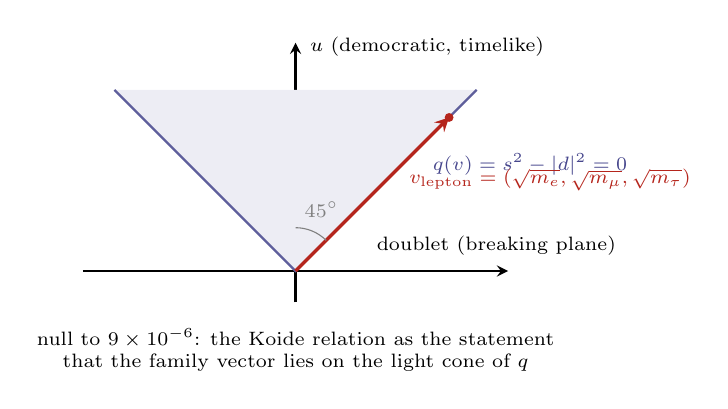
\begin{tikzpicture}[scale=1.0, >=stealth]
% face space as Minkowski: democratic axis vertical (timelike)
\draw[->, thick] (0,-0.4) -- (0,2.9);
\node[font=\scriptsize, anchor=west] at (0.06,2.85) {$u$ (democratic, timelike)};
\draw[->, thick] (-2.7,0) -- (2.7,0);
\node[font=\scriptsize, anchor=south] at (2.55,0.08) {doublet (breaking plane)};
% light cone at 45 degrees
\fill[MidnightBlue!8] (0,0) -- (2.3,2.3) -- (-2.3,2.3) -- cycle;
\draw[MidnightBlue!70, thick] (-2.3,2.3) -- (0,0) -- (2.3,2.3);
\node[MidnightBlue!80, font=\scriptsize, anchor=west] at (1.62,1.35)
  {$q(v) = s^{2} - |d|^{2} = 0$};
% the lepton vector on the cone
\draw[very thick, ->, BrickRed] (0,0) -- (1.95,1.95);
\fill[BrickRed] (1.95,1.95) circle (1.6pt);
\node[BrickRed, font=\scriptsize, anchor=north west] at (1.32,1.42)
  {$v_{\mathrm{lepton}} = (\sqrt{m_{e}}, \sqrt{m_{\mu}}, \sqrt{m_{\tau}})$};
% the 45 degree angle mark
\draw[gray] (0,0.55) arc (90:45:0.55);
\node[gray, font=\scriptsize] at (0.33,0.78) {$45^{\circ}$};
% annotation below
\node[font=\scriptsize, align=center] at (0,-1.0)
  {null to $9 \times 10^{-6}$: the Koide relation as the statement\\
   that the family vector lies on the light cone of $q$};
\end{tikzpicture}
\caption{The Koide relation as nullity (Proposition \ref{prop:nullity}). Face space, with $s = v \cdot u$ the singlet coordinate of a vector $v$ along the democratic unit vector $u$ and $d = v - su$ its doublet part, read through the Minkowski member $q(v) = s^{2} - |d|^{2}$ of the $S_{3}$-invariant forms, is a three-dimensional Minkowski space whose timelike axis is the democratic direction; the equal singlet-doublet split $s^{2} = |d|^{2}$ is its light cone, and the measured charged-lepton $\sqrt{m}$ vector lies on it to three parts in $10^{6}$. The member $q$ is a choice, not a consequence of the bracket geometry (Proposition \ref{prop:chart}): what the picture shows is Foot's $45^{\circ}$ in the vocabulary in which being null is the definition of being a point. What the framework does and does not supply for the relation is Section \ref{sec:gaussian}'s twofold conclusion.}
\label{fig:lightcone}
\end{figure}

\begin{proposition}[The chart computation: the sign twist, the bracket form, and the Fourier coordinates]\label{prop:chart}
Face space has a concrete realisation: the three $\omega$-spinors lie in the two-dimensional $S_{\omega}$, so the face vector of pairwise brackets $\Omega = ([\omega^{2}\omega^{3}], [\omega^{3}\omega^{1}], [\omega^{1}\omega^{2}])$ is the vector of $2 \times 2$ minors of a $3 \times 2$ array. Three consequences.
\begin{enumerate}
\item \emph{(The sign twist.)} Under an odd permutation of the twistor labels, $\Omega \mapsto -P\,\Omega$: the face vector transforms in $\mathbf{3} \otimes \mathrm{sgn} = \mathrm{sgn} \oplus \mathbf{2}$. The democratic direction is the sign representation, invariant as a line and odd as a vector, consistent with Proposition \ref{prop:alignment}'s language (a direction, not a vector) and tying the line's two orientations to the $S_{3}$-odd structure the ordering must break.
\item \emph{(The bracket form, and what it selects.)} The complex-bilinear form on face space built from the symplectic $\varepsilon$ on the spinor slots and the Kronecker $\delta$ on the family slots is $C(\Omega) = \sum_{k}\Omega_{k}^{2}$ (the letter is the series' for this form; it is not the Casimir $C$ of Fact \ref{fact:dictionary}), the Cauchy-Binet norm of the minors. It is $S_{3}$-invariant, and it is the member $\alpha = 1$, $\beta = -1$ of Proposition \ref{prop:nullity}'s family: on a real face vector $C(v) = s^{2} + |d|^{2} = |v|^{2}$, Euclidean, and $C(v_{\mathrm{lepton}}) = \sum_{k} m_{k} = 1883$ MeV, not zero. The $S_{3}$-invariant tensors on the family indices are $\delta_{kl}$ and the all-ones $J_{kl}$, so $C$ is singled out among the invariant forms only by excluding $J$, that is by requiring invariance under $O(3)$ on family indices rather than $S_{3}$, which nothing in the paper supplies. On the complexified doublet $C$ is nondegenerate, so, like every nondegenerate two-dimensional complex quadratic space, it is a hyperbolic plane: $C(f_{\pm}) = 0$ and $C(f_{+}, f_{-}) = 3$ for the Fourier vectors $f_{\pm} = (1, \zeta^{\pm 1}, \zeta^{\mp 1})$, $\zeta = e^{2\pi i/3}$, and $C(af_{+} + bf_{-}) = 6ab$, so its null vectors are exactly the two Fourier lines. Those lines contain no nonzero real vector: $C$-nullity and the $q$-nullity of Proposition \ref{prop:nullity} share nothing but the word.
\item \emph{(The Fourier coordinates, and the one number.)} The map $\Gamma \mapsto (\mathrm{Re}(\Gamma\zeta^{k}))_{k}$ is an $\R$-linear bijection from $\C$ onto the real doublet plane $\{d : \sum_{k} d_{k} = 0\}$, so every real face vector has the form
\begin{equation}\label{eq:parametrisation}
\sqrt{m_{k}} \;=\; a + |\Gamma|\cos\!\Bigl(\delta + \frac{2\pi k}{3}\Bigr), \qquad \delta = \arg\Gamma,
\end{equation}
three real parameters for three components: the classic Koide parametrisation, with its $2\pi/3$ phase spacing, is the Fourier coordinate system on $\mathbb{Z}/3$ and carries no hypothesis. In these coordinates the relation's entire content is one number: $Q_{\sqrt{m}} = \tfrac23 \iff |\Gamma|^{2} = 2a^{2}$, and the charged-lepton data give $|\Gamma|/a = 1.4142$ against $\sqrt{2} = 1.4142$ (the script certifies $|\Gamma|^{2}/a^{2} = 6Q_{\sqrt{m}} - 2$ inside $2 \pm 10^{-4}$), with $\delta = 0.222$ the free phase that encodes $m_{\mu}/m_{e}$, for the labelling $k = 0, 1, 2 = \tau, e, \mu$. The normalisation $|\Gamma|^{2} = 2a^{2}$, the one number, is Section \ref{sec:gaussian}'s question.
\end{enumerate}
\end{proposition}

\begin{proof}
(1) An odd permutation of the labels $\{1,2,3\}$ permutes the three brackets and flips each bracket's sign (each $[\omega^{i}\omega^{j}]$ is antisymmetric in $ij$), which is the displayed twist; $\mathbf{3} \otimes \mathrm{sgn}$ decomposes as stated. (2) Contracting the two spinor indices of $\Omega_{k}\Omega_{l}$ with $\varepsilon$ and the family indices with $\delta$ gives $\sum_{k}\Omega_{k}^{2}$; by Cauchy-Binet this is $\det(W^{\mathsf{T}}W)$ for the $3 \times 2$ array $W$. $S_{3}$-invariance is that of $\delta_{kl}$ (the twist squares to one), and the invariant-tensor count is the count of orbits of $S_{3}$ on pairs of indices, two: the diagonal and the off-diagonal, spanned by $\delta$ and $J - \delta$, equivalently by $\delta$ and the all-ones $J$. On real vectors $\sum_{k}v_{k}^{2} = |v|^{2} = s^{2} + |d|^{2}$. The evaluations: $C(f_{\pm}) = \sum_{k}\zeta^{\pm 2k} = 0$ (a full period sums to zero, since $\zeta^{2}$ is again a primitive cube root), $C(f_{+}, f_{-}) = \sum_{k}1 = 3$, and $C(af_{+} + bf_{-}) = a^{2}C(f_{+}) + b^{2}C(f_{-}) + 2ab\,C(f_{+}, f_{-}) = 6ab$, zero iff $a = 0$ or $b = 0$. A real vector on the $f_{+}$ line would satisfy $\Gamma\zeta^{k} \in \R$ for all $k$, forcing $\Gamma = 0$. (3) $\sum_{k}\mathrm{Re}(\Gamma\zeta^{k}) = \mathrm{Re}(\Gamma\sum_{k}\zeta^{k}) = 0$, so the image lies in the doublet plane; the map is $\R$-linear and injective ($\mathrm{Re}(\Gamma\zeta^{k}) = 0$ for $k = 0, 1$ forces $\Gamma = 0$), and both sides are two-dimensional over $\R$. With $\Gamma = |\Gamma|e^{i\delta}$ the components are \eqref{eq:parametrisation}. For the one number: $\sum_{k}\sqrt{m_{k}} = 3a$ and $\sum_{k}m_{k} = 3a^{2} + \tfrac32|\Gamma|^{2}$ (the cosines sum to zero and their squares to $\tfrac32$), so $Q_{\sqrt{m}} = \tfrac13 + |\Gamma|^{2}/(6a^{2})$, equal to $\tfrac23$ iff $|\Gamma|^{2} = 2a^{2}$. Every evaluation, including the cube-root sums as exact cyclotomic arithmetic (the script represents $\zeta$ by its minimal polynomial $\zeta^{2} + \zeta + 1 = 0$ over the rationals), the Euclidean identity $C(v) = |v|^{2}$ on the lepton vector, the Fourier bijection on explicit vectors, and the ratio $|\Gamma|^{2}/a^{2}$ bracketed against $2$ on the lepton data, is machine-verified.
\end{proof}

\section{The Gaussian theorems}\label{sec:gaussian}

The chain of Section \ref{sec:koide} reduces the Koide relation to one normalisation, and the way to fix a normalisation is to compute the vacuum. This section does the computation in the simplest class that has a vacuum to compute: the Gaussian one. The model, stated once. The six-mode face algebra has bosonic modes $a_{iA}$, $i \in \{1,2,3\}$ a family slot and $A \in \{1,2\}$ a spinor component; the face operators are the bracket quadratics
\[
\hat\Omega_{k} \;=\; \varepsilon_{AB}\,a_{iA}\,a_{jB} \;=\; \tfrac12\,\varepsilon_{kij}\,\varepsilon_{AB}\,a_{iA}a_{jB}, \qquad (i,j) \text{ the cyclic successors of } k,
\]
the operator form of Proposition \ref{prop:chart}'s minors. The frozen vacuum is the squeezed vacuum (Fact \ref{fact:gaussian}) of a pairing in the antisymmetric sector,
\[
\xi \;=\; \tau\,\bigl(G \otimes \varepsilon\bigr), \qquad G = [a]_{\times}, \qquad a = a_{A} + \lambda e^{i\chi}a_{B},
\]
where a family wedge $p \wedge q$ acts on the family space as the cross-product matrix $[p \times q]_{\times}$ and the two channels are the wedges $f_{+} \wedge f_{-}$, the $S_{3}$-safe channel available to the uncaused vacuum, with $a_{A} = f_{+} \times f_{-}$ normalised, and $u' \wedge f_{+}$, $u' = (1,1,1)$, the channel that uses the descent's orientation bit, with $a_{B} = u' \times f_{+}$ normalised; $\tau > 0$ is the strength, $\lambda \ge 0$ the feeding ratio, $\chi$ the channel phase, and $\lambda = 1$ the universal-strength point. The reading is the gauge-invariant symmetric square, forced by the bracket's gauge phase and the mass paper's $m^{2} = 2|B_{\Lambda}|^{2}$: the mass form is
\[
H_{kl} \;=\; \tfrac12\,\bigl\langle \hat\Omega_{k}^{\dagger}\hat\Omega_{l} + \hat\Omega_{l}\hat\Omega_{k}^{\dagger}\bigr\rangle,
\]
and the physical families are its eigenvectors, per Proposition \ref{prop:alignment}(3). Throughout, $r$ is the freezing depth (the common Takagi value of the pairing, Proposition \ref{prop:rigidity}), $x = \sinh^{2}r$, and $s = \sinh r$, $c = \cosh r$.

\begin{proposition}[Rigidity: the pairing sector is one event]\label{prop:rigidity}
Every pairing the descent can write in the antisymmetric sector, any complex combination of the channels at any strengths, has family factor $G = [a]_{\times}$, the cross-product matrix of some complex $3$-vector $a$, and
\begin{equation}\label{eq:gram}
G G^{\dagger} \;=\; |a|^{2}\,\mathbb{1} \;-\; \bar{a}\,a^{\mathsf{T}}, \qquad \mathrm{spec} = \{\,|a|^{2},\ |a|^{2},\ 0\,\},
\end{equation}
doubly degenerate identically in $a$. Consequently the Takagi spectrum of the full pairing is fourfold degenerate at every $(\lambda, \chi)$, $\{\sigma, \sigma, \sigma, \sigma, 0, 0\}$ with $\sigma = \tau|a|$; the freezing is exactly one Bogoliubov event with one depth $r = \sigma$, which for the two channels is $r = \tau\sqrt{1 + \lambda^{2}}$ ($\lambda$ is a relabelling of $\tau$ plus a rotation of the coherent ray); the equal-gain identity of the two channels holds to all orders; and the coherent face vector is
\[
v_{k} \;=\; \langle \hat\Omega_{k}\rangle \;=\; 2\,\sinh r\cosh r\;n_{k}, \qquad n = a/|a|,
\]
which at the universal point reads $v_{k} = -i\sqrt{\tfrac{2}{3}}\,\sinh r\cosh r\,\bigl(1 + e^{i\chi}\zeta^{k}\bigr)$ and in general $v_{k} \propto 1 + \lambda e^{i\chi}\zeta^{k}$.
\end{proposition}

\begin{proof}
A family wedge $p \wedge q$ acts on the three-dimensional family space as the antisymmetric matrix $[p \times q]_{\times}$, and every antisymmetric $3 \times 3$ matrix is $[a]_{\times}$ for a unique $a$, so complex combinations of the channels' wedges are of the stated form. The identity \eqref{eq:gram}: $([a]_{\times}w)_{i} = \varepsilon_{ijk}a_{j}w_{k}$ and $[a]_{\times}^{\dagger} = -[\bar a]_{\times}$, so $GG^{\dagger}w = -a \times (\bar a \times w) = |a|^{2}w - \bar{a}\,(a \cdot w)$ by the triple-product identity, which is \eqref{eq:gram}. Its spectrum: on the two-dimensional space $\{w : a \cdot w = 0\}$, the Hermitian orthogonal complement of $\bar a$, the second term vanishes, eigenvalue $|a|^{2}$ twice; and $GG^{\dagger}\bar{a} = |a|^{2}\bar{a} - \bar{a}\,(a \cdot \bar{a}) = 0$ since $a \cdot \bar{a} = |a|^{2}$, the exact zero. Tensoring with the spinor $\varepsilon$ (unitary, $2 \times 2$) gives $\xi\xi^{\dagger} = \tau^{2}\,GG^{\dagger} \otimes \mathbb{1}$, so the singular values of $\xi$, which are its Takagi values, are $\{\sigma, \sigma, \sigma, \sigma, 0, 0\}$ with $\sigma = \tau|a|$, fourfold degenerate for every channel combination. The two channels: $f_{+} \times f_{-} = (\zeta^{2} - \zeta)(1,1,1)$ and $u' \times f_{+} = (\zeta^{2} - \zeta)f_{+}$ with $\zeta^{2} - \zeta = -i\sqrt{3}$, so the normalised channel vectors are $a_{A} = -i(1,1,1)/\sqrt{3}$ and $a_{B} = -if_{+}/\sqrt{3}$, Hermitian-orthogonal ($\sum_{k}\zeta^{k} = 0$), whence $|a|^{2} = 1 + \lambda^{2}$ and $r = \tau\sqrt{1+\lambda^{2}}$. Because the nonzero Takagi values coincide, every function of the pairing applied in the Takagi basis (Fact \ref{fact:gaussian}) is a scalar multiple of $\xi$ on its range: $M = -\tfrac{\sinh\sigma\cosh\sigma}{\sigma}\,\xi = -sc\,\hat\xi$ with $\hat\xi = \xi/\sigma$, and $N = s^{2}\,\overline{\Pi}$ with $\Pi = \hat\xi\hat\xi^{\dagger} = R \otimes \mathbb{1}$, $R = \mathbb{1} - \bar{n}n^{\mathsf{T}}$ the projector onto $\{w : a \cdot w = 0\}$; this is the all-orders equal-gain statement, since both channels are fed through the same scalar. The coherent vector: $\langle\hat\Omega_{k}\rangle = \sum_{pq}\Theta_{k}[p,q]M_{pq}$ with $\Theta_{k} = \tfrac12(E_{k} \otimes \varepsilon)$, $(E_{k})_{ij} = \varepsilon_{kij}$, so $\langle\hat\Omega_{k}\rangle = -\tfrac{sc}{2|a|}\,\mathrm{tr}(E_{k}G)\,\mathrm{tr}(\varepsilon\varepsilon) = \tfrac{sc}{|a|}\,\mathrm{tr}(E_{k}G) = 2sc\,a_{k}/|a|$, using $\mathrm{tr}(\varepsilon\varepsilon) = -2$ and $\mathrm{tr}(E_{k}[a]_{\times}) = \sum_{ij}\varepsilon_{kij}\varepsilon_{jmi}a_{m} = 2a_{k}$. At the universal point $n = (a_{A} + e^{i\chi}a_{B})/\sqrt{2} = -i(1 + e^{i\chi}\zeta^{k})/\sqrt{6}$, which is the displayed formula. The spectrum identity \eqref{eq:gram}, the channel cross products, the orthogonality, and the coherent-vector formula are verified by the script in exact cyclotomic arithmetic.
\end{proof}

\begin{theorem}[The skeleton: rank one plus the ordering shift, and the unbreakable $S_{2}$]\label{thm:skeleton}
For every pairing of the antisymmetric sector, at every strength, feeding ratio and channel phase, the mass form evaluates in closed form:
\begin{equation}\label{eq:H}
H_{kl} \;=\; \cosh^{2}r\;\delta_{kl} \;+\; x(5+6x)\,\bar{n}_{k}n_{l},
\qquad
\mathrm{spec}\,H \;=\; \bigl(\cosh^{2}r,\ \cosh^{2}r,\ 1 + 6x + 6x^{2}\bigr),
\end{equation}
with $\bar{n}n^{\mathsf{T}} =: P_{[\bar{v}]}$ the projector onto the conjugate coherent ray, and the trace identity $\tr H = 3 + 8x + 6x^{2}$ tying it to the diagonal reading. Three clauses.
\begin{enumerate}
\item \emph{(Rank one plus floor.)} The normal-ordered form $\langle\hat\Omega_{k}^{\dagger}\hat\Omega_{l}\rangle$ is exactly $2x(2+3x)\,P_{[\bar v]}$, rank one: one heavy family along the conjugate coherent ray with the light pair strictly massless. Proposition \ref{prop:alignment}'s texture is a theorem of the Gaussian freezing at operator level.
\item \emph{(The floor is the ordering shift.)} The entire mass-squared of the light pair is the symmetric-ordering term $\tfrac12\langle[\hat\Omega_{l}, \hat\Omega_{k}^{\dagger}]\rangle = \cosh^{2}r\,\delta_{kl} + x\,P_{[\bar v]}$ restricted to the light plane, exactly $\cosh^{2}r$: the ordering shift, evaluated at depth $r$; that this is the same half-per-mode structure that determines $\hbar$ in the series is a reading, with the series' ordering dictionary \cite[Thm.~5.7]{ButlerT9} as its locator, and not part of the proved content. The light families' masses are the ordering shift alone.
\item \emph{(The $S_{2}$ is unbreakable in the class.)} The spectrum depends on the pairing only through the depth $r$ (Proposition \ref{prop:rigidity}); the channel phase and, at fixed $r$, the feeding ratio move only the coherent ray, and the light-pair degeneracy is exact for every pairing of the sector. Everywhere in the antisymmetric Gaussian class, $m_{e} = m_{\mu}$ identically: the $S_{2} \to 1$ stage of the cascade provably lies outside the Gaussian freezing.
\end{enumerate}
\end{theorem}

\begin{proof}
Write $\hat\Omega_{k} = \sum_{pq}\Theta_{k}[p,q]\,a_{p}a_{q}$ with $\Theta_{k} = \tfrac12(E_{k} \otimes \varepsilon)$ symmetric and real, and put $\omega_{k} = \langle\hat\Omega_{k}\rangle = \mathrm{tr}(\Theta_{k}M)$. By Wick's theorem (Fact \ref{fact:gaussian}), using the symmetry of $\Theta_{l}$ to merge the two $NN$ terms,
\[
\langle\hat\Omega_{k}^{\dagger}\hat\Omega_{l}\rangle = 2\,\mathrm{tr}\bigl(\Theta_{k}N\Theta_{l}N^{\mathsf{T}}\bigr) + \bar\omega_{k}\omega_{l}, \qquad
\langle\hat\Omega_{l}\hat\Omega_{k}^{\dagger}\rangle = 2\,\mathrm{tr}\bigl(\Theta_{l}(\mathbb{1}+N^{\mathsf{T}})\Theta_{k}(\mathbb{1}+N)\bigr) + \omega_{l}\bar\omega_{k},
\]
so that
\[
H_{kl} \;=\; \bar\omega_{k}\omega_{l} + \mathrm{tr}(\Theta_{l}\Theta_{k}) + \mathrm{tr}(\Theta_{k}\Theta_{l}N^{\mathsf{T}}) + \mathrm{tr}(\Theta_{l}\Theta_{k}N) + 2\,\mathrm{tr}(\Theta_{k}N\Theta_{l}N^{\mathsf{T}}),
\]
four pieces. Insert the Gaussian data of Proposition \ref{prop:rigidity}: $N = s^{2}\,\overline{R} \otimes \mathbb{1}$, $N^{\mathsf{T}} = s^{2}\,R \otimes \mathbb{1}$ with $R = \mathbb{1} - \bar{n}n^{\mathsf{T}}$, and $\omega_{k} = 2sc\,n_{k}$. Every trace factorises over the tensor product, with $\mathrm{tr}(\varepsilon\varepsilon) = -2$ on the spinor factor, and on the family factor the only identities needed are $E_{k}E_{l} = e_{l}e_{k}^{\mathsf{T}} - \delta_{kl}\mathbb{1}$ (from $\sum_{j}\varepsilon_{kij}\varepsilon_{ljm} = \delta_{km}\delta_{il} - \delta_{kl}\delta_{im}$), hence $\mathrm{tr}(E_{k}E_{l}) = -2\delta_{kl}$ and $\mathrm{tr}(E_{k}E_{l}X) = X_{kl} - \delta_{kl}\,\mathrm{tr}X$, and $n^{\mathsf{T}}E_{k}n = 0$ (antisymmetry). The pieces:
\begin{align*}
\mathrm{tr}(\Theta_{l}\Theta_{k}) &= \tfrac14\,\mathrm{tr}(E_{l}E_{k})\,\mathrm{tr}(\varepsilon\varepsilon) = \delta_{kl},\\
\mathrm{tr}(\Theta_{k}\Theta_{l}N^{\mathsf{T}}) + \mathrm{tr}(\Theta_{l}\Theta_{k}N) &= -\tfrac{s^{2}}{2}\bigl[\mathrm{tr}(E_{k}E_{l}R) + \mathrm{tr}(E_{l}E_{k}\overline{R})\bigr]\\
&= -\tfrac{s^{2}}{2}\bigl[(R_{kl} - 2\delta_{kl}) + (\overline{R}_{lk} - 2\delta_{kl})\bigr] = s^{2}\delta_{kl} + s^{2}\,\bar{n}_{k}n_{l},\\
2\,\mathrm{tr}(\Theta_{k}N\Theta_{l}N^{\mathsf{T}}) &= -s^{4}\,\mathrm{tr}(E_{k}\overline{R}E_{l}R)\\
&= -s^{4}\bigl[-2\delta_{kl} - (n_{l}\bar{n}_{k} - \delta_{kl}) - (\bar{n}_{k}n_{l} - \delta_{kl}) + (n^{\mathsf{T}}E_{k}n)(\bar{n}^{\mathsf{T}}E_{l}\bar{n})\bigr]\\
&= 2s^{4}\,\bar{n}_{k}n_{l},\\
\bar\omega_{k}\omega_{l} &= 4s^{2}c^{2}\,\bar{n}_{k}n_{l},
\end{align*}
using $\mathrm{tr}\,R = 2$, $\overline{R}_{lk} = R_{kl}$, and in the third line the expansion of $\overline{R} = \mathbb{1} - n\bar{n}^{\mathsf{T}}$ and $R = \mathbb{1} - \bar{n}n^{\mathsf{T}}$ into four traces. Summing, $H_{kl} = (1 + s^{2})\delta_{kl} + (s^{2} + 2s^{4} + 4s^{2}c^{2})\,\bar{n}_{k}n_{l} = c^{2}\delta_{kl} + x(5 + 6x)\,\bar{n}_{k}n_{l}$ with $c^{2} = 1 + x$, which is \eqref{eq:H}; the heavy eigenvalue is $1 + x + 5x + 6x^{2}$ and the trace is $3(1+x) + 5x + 6x^{2}$. The normal-ordered form is the first and last pieces of $\langle\hat\Omega_{k}^{\dagger}\hat\Omega_{l}\rangle$ alone, $2s^{4}\bar{n}_{k}n_{l} + 4s^{2}c^{2}\bar{n}_{k}n_{l} = 2x(2+3x)\,\bar{n}_{k}n_{l}$, rank one, which is clause (1); the ordering term is the remainder, $c^{2}\delta_{kl} + x\bar{n}_{k}n_{l}$, whose restriction to the light plane is $c^{2}$, clause (2); and clause (3) is the statement that \eqref{eq:H} depends on the pairing only through $r$ and the ray $n$. The script evaluates the four pieces and their sum in exact cyclotomic arithmetic, from the Wick formula and the Gaussian data, at rational hyperbolic points $(s, c) = (\tfrac34, \tfrac54), (\tfrac{12}{5}, \tfrac{13}{5})$, feeding ratios $\lambda \in \{0, \tfrac34, \tfrac43\}$ (chosen so that $|a|$ is rational) and channel phases $e^{i\chi} \in \{1, \zeta, \zeta^{2}\}$, and confirms each piece against its closed form and the total against \eqref{eq:H}; the trace and eigenvalue identities are checked as rational-function identities in $x$.
\end{proof}

\begin{proposition}[Koide in the class: the crossing, and the fit conclusion]\label{prop:crossing}
Within the Gaussian class the only Koide-compatible configuration is the $S_{2}$-symmetric point (one heavy, two exactly degenerate light), where the relation reduces to a single ratio: $Q_{\sqrt{m}} = 2/3$ for the mass triple $(t, t, T)$ holds iff $\sqrt{T/t} = 4 + 3\sqrt{2}$, equivalently a heavy-to-light mass-squared ratio of $K = (4+3\sqrt{2})^{4} = 2308 + 1632\sqrt{2} \approx 4616$. In the model's variables the condition is
\begin{equation}\label{eq:crossing}
\frac{1 + 6x + 6x^{2}}{1 + x} \;=\; 6x + \frac{1}{1+x} \;=\; K,
\end{equation}
which the depth crosses exactly once, at $x^{*} = \sinh^{2}r^{*} = K/6 - 1/(6(1 + x^{*})) = 769.3325$, within $2.2 \times 10^{-4}$ of $K/6 = 769.3328$. The conclusion: the depth is not canonical; $x^{*}$ is $K/6$ up to the $1/(6(1+x))$ term because the skeleton's ratio is $6x$ at large depth, so the depth is Koide's own number transcribed by the spectrum of \eqref{eq:H}, and two parameters (depth and scale) against two observables is a reparametrisation, not a mechanism. \textbf{The mechanism stands as a fit; the derivation claim is refuted at this order.} The relation reverts, within the framework as it stands, to a measurement: of the freezing depth, at $10^{-5}$ precision.
\end{proposition}

\begin{proof}
The reduction at the $S_{2}$ point: for $\sqrt{m}$-triple $(\sqrt{t}, \sqrt{t}, \sqrt{T})$, $Q = (2t + T)/(2\sqrt{t} + \sqrt{T})^{2} = 2/3$ rearranges to $\rho^{2} - 8\rho - 2 = 0$ for $\rho = \sqrt{T/t}$, whose positive root is $4 + \sqrt{18} = 4 + 3\sqrt{2}$; in the Fourier coordinates of Proposition \ref{prop:chart}(3) the $S_{2}$ point is $\delta = 0$ with $\sqrt{m} = (a + |\Gamma|, a - |\Gamma|/2, a - |\Gamma|/2)$, and at $|\Gamma| = a\sqrt{2}$ the ratio $(a + |\Gamma|)/(a - |\Gamma|/2) = (1 + \sqrt{2})(2 + \sqrt{2}) = 4 + 3\sqrt{2}$, the same root; the fourth power evaluates in $\mathbb{Z}[\sqrt{2}]$ as $(4+3\sqrt{2})^{2} = 34 + 24\sqrt{2}$ and $(34+24\sqrt{2})^{2} = 2308 + 1632\sqrt{2}$. The middle form of \eqref{eq:crossing} is the division $6x^{2} + 6x + 1 = 6x(1+x) + 1$; it is strictly increasing in $x > 0$ (derivative $6 - 1/(1+x)^{2} > 0$), which gives the single crossing and the displayed identity for $x^{*}$. The script brackets $x^{*}$ between rational bounds by exact sign evaluation in $\mathbb{Z}[\sqrt{2}]$ arithmetic, $769.332 < x^{*} < 769.333$, and confirms $K/6 - x^{*} \in (2 \times 10^{-4}, 3 \times 10^{-4})$. The conclusion clause is the paper's pre-registered refutation condition for a canonical depth, applied: the nominated canonical depth fails by orders of magnitude ($\tanh^{2}r = \tfrac12$, that is $x = 1$, gives a ratio of $13/2$), and no independent structure marks $x^{*}$.
\end{proof}

\begin{proposition}[The classification: the displaced-Gaussian class is solved, at the level of its weakest clause]\label{prop:classification}
The candidate inventory for the $S_{2} \to 1$ splitting within the displaced-Gaussian class of the six-mode face algebra has three entries, of which the first is closed by theorem and the other two by flagged preliminary computation:
\begin{enumerate}
\item \emph{(More pairing channels: closed by theorem.)} By Proposition \ref{prop:rigidity} and Theorem \ref{thm:skeleton}, every antisymmetric pairing is one fourfold-degenerate event with an exactly degenerate light pair. No pairing the descent can write splits the degenerate pair.
\item \emph{(The symmetric-spinor noise channel: preliminary computation.)} Preliminary computation by the methods of this section, in a displaced-Gaussian computation checked against exact Fock-space evaluation, indicates that the one pairing outside the $\varepsilon$-sector splits the pair but cannot reach the physical ratio pair $(m_{\mu}/m_{e}, m_{\tau}/m_{\mu}) = (206.77, 16.82)$: the best attainable point found is $(101, 19)$, far from Koide, with the deformation of $Q$ excluding the route along the way. The scan is not reproduced by this paper's script and the clause carries that level.
\item \emph{(The condensate means: preliminary computation.)} The same computation indicates that nonzero means with the flag-forced equal-amplitude form cap the split at $1.2032$, short of $206.77$ by a factor of $172$; and that with free amplitudes the physical spectrum is reachable exactly at every depth, with the solution itself showing why: the required leg asymmetry is $g_{1}/g_{2} \approx 207.5$, the muon-electron ratio relabelled, with sensitivity of the predicted split to the free parameter exactly $1$ and the heavy mass not responding at all. A mechanism whose parameters are the answer derives nothing. Same level as (2).
\end{enumerate}
The terminal statement, at the level of its weakest clause: the displaced-Gaussian class is solved; its entire output is the rank-one-plus-shift skeleton (rigidly one event, $S_{2}$-exact, by theorem), bounded Koide-incompatible perturbations of it, and free mean textures that are the mass data under another name. The physical charged-lepton spectrum lies in the class only as a relabelling of itself. The remaining route is named and constrained: a non-Gaussian frozen vacuum or a larger algebra, required to produce the number $207$ from caused structure, with the relabelling signature (unit sensitivity to a free parameter) as the refutation condition on every future candidate.
\end{proposition}

\begin{proof}
(1) is Proposition \ref{prop:rigidity} with Theorem \ref{thm:skeleton}: the light eigenvalue $\cosh^{2}r$ is doubly degenerate for every $a$. (2) and (3) are not proved here; they are the results of a displaced-Gaussian computation by the methods of Theorem \ref{thm:skeleton} extended to the symmetric-spinor pairing and to nonzero means, reported at their stated level with the numbers they returned, and the classification sentence is the conjunction of the three clauses at the level of (2) and (3): the class's parameters are exactly (antisymmetric pairings, the symmetric noise pairing, means), and each is addressed. What is a theorem in the terminal statement is the skeleton and its unbreakable $S_{2}$; what is preliminary is the bound on the noise channel and the relabelling conclusion on the means, and the levels of the results record the distinction.
\end{proof}

\section{The terminal state}\label{sec:terminal}

\begin{observation}[One open problem in three forms]\label{obs:debt}
The flavour problem, in this framework and at the displaced-Gaussian state class, is not an undiscovered operator: it is the numbers layer, three times over. The split ($m_{\mu}/m_{e} \approx 207$), the angle ($45^{\circ}$, present only through the depth), and the depth ($x^{*} \approx 769$) are one open problem in three forms, and the Gaussian vacuum treats all three as inputs. The registered open problem is the non-Gaussian completion: structure beyond the class (a non-Gaussian frozen vacuum with higher cumulants, or a larger algebra) that produces the $207$ from caused structure, constrained by the relabelling-signature refutation condition of Proposition \ref{prop:classification}, and required to preserve the skeleton of Theorem \ref{thm:skeleton} and to introduce no second free number. Until it is solved, the Koide relation stands within the framework as what the chain of refutations has made it: a $10^{-5}$-precision measurement of a frozen vacuum whose structure is theorems and whose numbers remain to be derived.
\end{observation}

\begin{observation}[Koide as instrument]\label{obs:instrument}
Whatever the mechanism, the relation's observed exactness is a measurement of the frozen vacuum's face sector. By $Q_{v} = 1/(3\cos^{2}\theta)$, $\delta Q/Q = 2\tan\theta\,\delta\theta$, so at $\theta = 45^{\circ}$ the relative deviation $3.3 \times 10^{-6}$ of Proposition \ref{prop:linearkill} puts the angle of the $\sqrt{m}$ vector to the democratic axis at $45^{\circ}$ minus $1.7 \times 10^{-6}$ radians on the central masses, an exact-arithmetic consequence the script checks. The $\pm 0.09$ MeV on $m_{\tau}$ moves the angle by about $3.8 \times 10^{-6}$ radians, so the offset the instrument reads is below its resolution: the data are consistent with exactly $45^{\circ}$. Any mechanism that moves the singlet and doublet norms together leaves $\theta$ fixed and is invisible to the relation; what it measures is the differential effect on the two components. Whatever else it is, the relation is a precision instrument reading the frozen vacuum's face sector.
\end{observation}

\begin{observation}[Selectivity, at observation level]\label{obs:selectivity}
The quarks fail the relation at pole masses, and the framework contains the structural asymmetry a selective mechanism needs: under Hypothesis (S) the leptons are whole-twistor states, colour singlets whose brackets are physical masses undressed, while quarks are pair-level cells, their pole masses dressed by the strong interaction (Fact \ref{fact:generation}). The neutrinos are exempt structurally: their masses are seesaw-composed, quadratic again in the bracket-linear objects, so the null condition constrains the unobservable Dirac layer and imposes nothing on the physical $m_{\nu}$ (the neutrino paper T15 \cite{ButlerT15} carries the neutrino mass sector and does not treat the relation; the exemption is this paper's observation). Both statements are consistencies, not derivations, and are flagged at observation level; a genuine account would compute the dressing.
\end{observation}

\begin{observation}[The absolute scale: a clean negative result]\label{obs:absolute}
The other half of the weight problem, why $\mathrm{Im}\,w_{e} \sim 10^{38}$ at all (Fact \ref{fact:dictionary}), resists every structural attack attempted: expressing the imaginary weights as powers of $N$ finds no clean exponent for the electron or the weak scale, and the one suggestive scaling (a hadronic weight $\mathrm{Im}\,w_{h} \sim N^{2/3}$ with $N = M_{P}/H$ of Fact \ref{fact:moduli}, equivalently $m_{h} \sim (M_{P}^{2}H)^{1/3} \approx 5 \times 10^{7}$ eV on the inputs of Proposition \ref{prop:alignment}(1), the pion-scale coincidence) reduces to the Zel'dovich-Weinberg coincidence, in the literature since 1967 \cite{Zeldovich1967, Weinberg1972}, and therefore fails the series' prior-art condition. Counting the tower's hyperbolic pairs, mode-count ratios, and fine-structure powers all fail their own refutation conditions. The absolute hierarchy remains as the fifth and thirteenth refutations left it: one unexplained number, restated, with a map of the routes that do not work.
\end{observation}

\begin{proposition}[Why the kinematic attacks had to fail]\label{prop:covariance}
On the principal series $w = -\tfrac32 \pm i\nu$ with $\nu = m/H + O(H/m)$ (Fact \ref{fact:dictionary}), so that $\mathrm{Im}\,w$ is the mass in Hubble units and, trivially,
\[
\mathrm{Im}\,w \;=\; \frac{m}{H} \;=\; N \cdot \frac{m}{M_{P}} .
\]
Under the rescaling of Fact \ref{fact:moduli}, $\Lambda \to \kappa^{2}\Lambda$ at fixed $M_{P}$, the two factors have different status: $N \to N/\kappa$, which is the proved clause of Fact \ref{fact:moduli}; and $m/M_{P}$ is invariant, $m$ fixed while $H \to \kappa H$, which is the observation-level reading of \cite[Prop.~7.6(1)]{ButlerT12} recorded in Fact \ref{fact:moduli} and is the premise of this proposition, so that the proposition stands at that level. Granting it, $\mathrm{Im}\,w \to \mathrm{Im}\,w/\kappa$, and consequently any relation $\mathrm{Im}\,w = f(N)$ that holds across the family of frozen points must satisfy $f(N/\kappa) = f(N)/\kappa$ for every $\kappa > 0$, which forces $f$ linear, $\mathrm{Im}\,w = cN$ with $c = m/M_{P}$ a rescaling invariant. A power law $\mathrm{Im}\,w \sim N^{a}$ with $a \neq 1$, the hadronic $N^{2/3}$ of Observation \ref{obs:absolute} or any other clean exponent, is the relation $m/M_{P} \sim N^{a - 1}$ between two independent continuous moduli of the kinematic layer, which by Fact \ref{fact:moduli} fixes neither. So no kinematic attack can give an exponent other than one, and the exponent one says only that $m/M_{P}$ is a number. The Zel'dovich-Weinberg coincidence, $m_{h}^{3} \sim M_{P}^{2}H$, is $m_{h}/M_{P} \sim N^{-1/3}$ and can be, in this framework, only a coincidence of the present epoch or a dynamical relation among couplings, never a kinematic theorem. The map of failed routes in Observation \ref{obs:absolute} is thereby closed by a proof rather than left open: the absolute scale dissolves into three separately assigned pieces, $N$ (the cosmological constant, behind the promotion decision and then the descent measure, the Standard-Model paper's successor (5)), the rung unit $v/M_{P} \approx 2 \times 10^{-17}$ (a second rescaling-invariant modulus, the Standard-Model paper's successor (1), so kinematically not a function of $N$), and the Yukawa pattern, $y_{e} \approx 3 \times 10^{-6}$ and the ratios (Section \ref{sec:weights}). Only the third has computable structure available; and the second-order breaking and the CKM angles, being ratios and angles, are invariant under the rescaling and independent of the first two, so they depend on the third alone.
\end{proposition}

\begin{proof}
The dictionary of Fact \ref{fact:dictionary} gives $m^{2} = -w(w+3)H^{2}$, so on $w = -\tfrac32 + i\nu$, $m^{2} = (\nu^{2} + \tfrac94)H^{2}$ and $\nu = m/H\,(1 + O(H^{2}/m^{2}))$; the factorisation is arithmetic, $m/H = (M_{P}/H)(m/M_{P})$. The transformation law is Fact \ref{fact:moduli}'s clause with $H^{2} = \Lambda/3$. Covariance: setting $g(N) = f(N)/N$, the condition reads $g(N/\kappa) = g(N)$ for all $\kappa$, so $g$ is constant. The script checks, as exact monomial identities in the exponents of $(H, M_{P}, m)$, that $\mathrm{Im}\,w = N\,(m/M_{P})$; that under the substitution $H \to \kappa H$ with $M_{P}$ and $m$ fixed, the premise, the factor $N$ carries weight $-1$ and $m/M_{P}$ weight $0$; and that a power law $cN^{a}$ satisfies the covariance, as an identity of monomials in $(N, \kappa)$ with $\kappa$ symbolic, exactly when $a = 1$, tested at $a = -\tfrac13, \tfrac13, \tfrac23, 1, 2$, the first being the Zel'dovich-Weinberg exponent, and again on rational instances at $\kappa = 2$ for $a = 1, 2$. The six logarithmic ratios $\log\mathrm{Im}\,w/\log N$ for the electron, muon, tau, pion, proton and weak scale on $H_{0} = 67.4$ km/s/Mpc, $0.63$, $0.67$, $0.69$, $0.67$, $0.69$, $0.73$, are printed by the script as RECORD lines; that they share no common exponent is the expected behaviour of an invariant times a modulus, and is recorded, not claimed. The statement about the breaking and the CKM angles is a reading of what depends on what.
\end{proof}


\section{The weight spectrum: the order of operations}\label{sec:weights}

The Standard-Model paper derives the tree relations $m_{\nu} = m_{u}$, $m_{e} = m_{d}$ from a vev in the rung directions of the $10$ and proves three no-go theorems on what can dress them \cite[Cor.~9.25, Thms.~9.31, 9.33, 9.35]{ButlerT12}. This section locates in the module the one direction that carries the second family's factor on a single family, records the grade-three direction that can carry it between families, and fixes the order of operations of the matter programme: the two-term structure first, the family breaking second, the order the capstone's table of open directions records \cite[Table~4]{ButlerT17}. Throughout, the module is the Standard-Model paper's two-rung module \cite[Def.~9.8]{ButlerT12}, realised on $\Lambda^{\bullet}\C^{5}$ with $v_{a}$ acting by wedge and $w_{a}$ by contraction, modes $1, 2, 3$ the pairs and $4, 5$ the rungs; $N_{W}$ and $N_{R}$ are the pair and rung number operators; the sixteen is the even subspace, and its species reading, $\nu^{c}, e^{c}, Q, L, u^{c}, d^{c}$ at (rungs, pairs) $= (0,0), (2,0), (1,1), (1,3), (0,2), (2,2)$, is the Standard-Model paper's under Hypothesis (S) \cite[Prop.~5.8]{ButlerT12}, so that every statement below naming a species carries (S); $B$ is the $\so(10)$-invariant bilinear pairing \cite[Lem.~9.23]{ButlerT12}; and for an odd element $T$ of the Clifford algebra of the ten, the \emph{mass form} is $Y_{T}(\psi, \varphi) = B(\psi, T\varphi)$ on the sixteen. The operator $B - L := 1 - \tfrac23 N_{W}$ takes the values $(1, 1, \tfrac13, -1, -\tfrac13, -\tfrac13)$ on $(\nu^{c}, e^{c}, Q, L, u^{c}, d^{c})$: $B - L$ is an affine function of the pair number (script). The decomposition of $16 \otimes 16$ and the dictionary between grades and $\mathrm{Spin}(10)$ representations are stated as Fact \ref{fact:decomp} at the end of the section.

\begin{proposition}[The $126$ doublet direction in the module, and the Georgi-Jarlskog Clebsch]\label{prop:126}
Let $\chi := -(-1)^{N_{R}}$, which is $+1$ on the doublet sector $N_{R} = 1$ and $-1$ on the singlet sectors $N_{R} \in \{0, 2\}$, and let
\[
T_{\mathrm{GJ}} \;:=\; w_{4}\,(B - L)\,\chi .
\]
Then:
\begin{enumerate}
\item[(i)] $B - L = -\tfrac23\sum_{i \le 3} v_{i}\wedge w_{i}$ is pure grade two, $w_{4}\,\chi = w_{4}(1 - 2n_{5}) = -2\,w_{4}\,(v_{5}\wedge w_{5})$, and
\[
T_{\mathrm{GJ}} \;=\; \tfrac43\; w_{4}\wedge (v_{5}\wedge w_{5}) \wedge \Bigl(\sum_{i\le 3} v_{i}\wedge w_{i}\Bigr),
\]
a pure grade-five element of the Clifford algebra of the ten, with no grade-one and no grade-three component; hence, by Fact \ref{fact:decomp}, it has no $10$ and no $120$ component, and the mass form it induces on the sixteen is the $126$ component of $16 \otimes 16$, the $\overline{126}$ part of the grade-five space acting as zero on the sixteen;
\item[(ii)] under Hypothesis (S), which supplies the species names, $Y_{T_{\mathrm{GJ}}}$ is symmetric, conserves hypercharge, and is nonzero exactly on $(L, e^{c})$ with entries $-1$ and on $(Q, d^{c})$ with entries $\pm\tfrac13$, in the normalisation in which the $10$ form $Y_{w_{4}}$ has entries $\pm1$ on the same pairs; writing $y_{e}$, $y_{d}$ for the entries of $Y_{T_{\mathrm{GJ}}}$ on $(L, e^{c})$ and $(Q, d^{c})$, the ratio $|y_{e}/y_{d}| = 3$ is Georgi-Jarlskog's, and it is the ratio of the lepton doublet's to the quark doublet's $B - L$;
\item[(iii)] the one-sided weighting $w_{4}(B - L)$ without $\chi$ is antisymmetric on every coupled pair and contributes no one-family mass, because every Yukawa pair is $B - L$ neutral, $(B-L)(L) + (B-L)(e^{c}) = 0 = (B-L)(Q) + (B-L)(d^{c})$;
\item[(iv)] under Hypothesis (S) as in (ii), the up-type direction $v_{4}(B - L)\chi$ has a symmetric mass form coupling $(L, \nu^{c})$ with modulus $1$ and $(Q, u^{c})$ with modulus $\tfrac13$, so that $|m_{\nu}^{D}| = 3\,|m_{u}|$ on the $126$ direction; the signed entries are $+1$ on $(L, \nu^{c})$ and $\pm\tfrac13$ on $(Q, u^{c})$, the sign depending on the colour of the pair, so the relation is one of magnitudes.
\end{enumerate}
\end{proposition}

\begin{proof}
(i): $N_{W} = \sum_{i\le3} v_{i}w_{i} = \sum_{i\le3}(v_{i}\wedge w_{i} + \tfrac12)$ since $v_{i}\cdot w_{i} = \tfrac12$, so $1 - \tfrac23 N_{W} = -\tfrac23\sum v_{i}\wedge w_{i}$. For the rung: $w_{4}(1 - 2v_{4}w_{4}) = w_{4} - 2(1 - v_{4}w_{4})w_{4} = -w_{4}$ using $w_{4}^{2} = 0$, so $w_{4}\chi = -w_{4}(1 - 2n_{4})(1 - 2n_{5}) = w_{4}(1 - 2n_{5}) = -2w_{4}(v_{5}\wedge w_{5})$. The three factors $w_{4}$, $v_{5}\wedge w_{5}$, $\sum v_{i}\wedge w_{i}$ are built from mutually orthogonal vectors ($w_{4}$ anticommutes with $v_{5}, w_{5}$ and with every pair vector; the rung plane is orthogonal to the pair space), so their Clifford product is their wedge and has grade $1 + 2 + 2 = 5$. The script verifies the operator identity $T_{\mathrm{GJ}} = \tfrac43 w_{4}(v_{5}\wedge w_{5})(\sum v_{i}\wedge w_{i})$ on the module, the anticommutations, and, independently, the grade decomposition of $T_{\mathrm{GJ}}$ by the trace formula in the orthonormal basis $a_{i} = v_{i} + w_{i}$, $b_{i} = v_{i} - w_{i}$ of $\Cl(5,5)$ (coefficient of the blade $\Gamma_{A}$ is $\mathrm{tr}(\Gamma_{A}^{-1}T)/32$, the blades being trace-orthogonal in the irreducible representation), finding grade five only. The last clause of (i) is Fact \ref{fact:decomp} applied to the map $T \mapsto Y_{T}$, which is $\mathrm{Spin}(10)$-equivariant because $B$ is invariant: the grade-five space is $126 \oplus \overline{126}$, the bilinear forms on the sixteen are $16 \otimes 16 = 10 \oplus 120 \oplus 126$, and the $\overline{126}$ component, having no isomorphic summand among them, is sent to zero by Schur's lemma. (ii): $Y_{T_{\mathrm{GJ}}}(\psi, \varphi) = B(\psi, w_{4}\varphi)\cdot(B - L)(\varphi)\chi(\varphi)$ since $B - L$ and $\chi$ are diagonal; on $(L, e^{c})$ the factor is $(B-L)(e^{c})\chi(e^{c}) = 1\cdot(-1)$ in one order and $(B-L)(L)\chi(L) = (-1)(+1)$ in the other, on $(Q, d^{c})$ it is $(-\tfrac13)(-1)$ and $(\tfrac13)(+1)$: equal in both orders, which is the symmetry, with the stated values times the $\pm1$ of $Y_{w_{4}}$. The script enumerates the form and checks symmetry and hypercharge conservation entry by entry. (iii): without $\chi$ the two orders carry $(B-L)(e^{c}) = 1$ and $(B-L)(L) = -1$, opposite signs; the script checks antisymmetry and the neutrality sums. (iv) is the same computation with $v_{4}$; the script enumerates the form, checks its symmetry, and records the signed entries, $+1$ on both $(L, \nu^{c})$ entries and $-\tfrac13$, $+\tfrac13$ on the $(Q, u^{c})$ entries according to colour, which is why only the magnitude is stated.
\end{proof}


\begin{fact}[imported: the tree relations, the family no-go, and the two other no-gos]\label{fact:nogos}
On the one-generation module, a vector $c = a v_{4} + b w_{4}$ of the rung plane has mass form with entries of magnitude $|a|$ on $(L, \nu^{c})$, $(Q, u^{c})$ and $|b|$ on $(L, e^{c})$, $(Q, d^{c})$, so at tree level $m_{\nu} = m_{u}$ and $m_{e} = m_{d}$, the relations of a single $10$; and three no-go theorems follow. (i) With the three families carried by a tensor factor on which the family structure acts by any matrix $F$, and with $y_{e}$, $y_{d}$ now denoting the entries of the $10$ form of $c$ on $(L, e^{c})$ and $(Q, d^{c})$, $M_{e} = y_{e}F$ and $M_{d} = y_{d}F$ with $|y_{e}| = |y_{d}|$ have identical spectra in magnitude for every $F$: no operation in family space, the breaking $S_{3} \to S_{2} \to 1$ included, produces $m_{\mu} \neq m_{s}$ or $m_{e} \neq m_{d}$ at tree level. (ii) The algebra generated by the frozen point and the rung components of its lifts is eight-dimensional and contains no colour-singlet doublet direction beyond the $10$. (iii) The algebra generated by the frozen point, its lifts, the mass bracket and its conjugate is thirty-two-dimensional, its colour-singlet part is the rung Clifford algebra, and every symmetric doublet mass form it produces is a multiple of the $10$ form. The observed second family needs $m_{\mu} \approx 3 m_{s}$ at the unification scale, the Georgi-Jarlskog factor \cite{GeorgiJarlskog1979}. \emph{Provenance:} \cite[Cor.~9.25, Thms.~9.31, 9.33, 9.35]{ButlerT12}, proved there on the module and conditional on Hypothesis (S) for the species reading; the factor three is the literature's, at record level.
\end{fact}

\begin{corollary}[The order of operations in the matter programme]\label{cor:order}
Under Hypothesis (S), which supplies the species names, the family breaking cannot come first: by Fact \ref{fact:nogos}(i) the family breaking acting on a $10$-vev leaves $m_{\mu} = m_{s}$ and $m_{e} = m_{d}$ exactly, and the observed second family needs the factor $3$ at the unification scale (Fact \ref{fact:nogos}). Among one-family mass forms the factor is available in the module as the direction of Proposition \ref{prop:126}, and only there: the symmetric doublet mass forms of odd colour-singlet elements with the doublet's charges span the two-dimensional space of the $10$ form and the $T_{\mathrm{GJ}}$ form \cite[Prop.~9.32]{ButlerT12}. With three families there is a second source, the one-sided weighting of Proposition \ref{prop:126}(iii), whose antisymmetric form gives no one-family mass but does give entries between families through an antisymmetric family coupling (Fact \ref{fact:gradethree}). That direction requires the electroweak vev to couple not as a bare rung vector but as the rung vector wedged with the other rung's area bivector and with the pair-sector $\uu(1)$ generator. So the first result required of the weight programme is not a family texture but a \emph{pair-number-dependent rung coupling}: a derivation, from the mass mechanism, of a term of the form $w_{4}\wedge(v_{5}\wedge w_{5})\wedge\sum v_{i}\wedge w_{i}$ alongside the bare $w_{4}$, with the ratio of the two coefficients then fixing $m_{\mu}/m_{s}$ and $m_{e}/m_{d}$ jointly (the third family is where the bare $10$ relation $m_{b} \approx m_{\tau}$ is approximately right). Both sources carry the pair-number current, so the requirement stands on the route the Standard-Model paper registers, where the second family's factor comes through mixing with the third by the grade-three source and the role of that ratio passes to the coupling between the two families (Fact \ref{fact:gradethree}). The family breaking is the second step, acting on the resulting two-term structure; this is the order the capstone's table of open directions records for the matter programme \cite[Table~4]{ButlerT17}.
\end{corollary}

\begin{proof}
Immediate from Fact \ref{fact:nogos}(i), Proposition \ref{prop:126}, the uniqueness statement of \cite[Prop.~9.32]{ButlerT12} and the imported factor, with Fact \ref{fact:gradethree} for the three-family sentences; the last clause is the standard reading of the Georgi-Jarlskog relation and is recorded at that level. The family breaking of Sections \ref{sec:koide} and \ref{sec:gaussian} is unaffected by this: it acts on whichever two-term structure the mass mechanism supplies, and the modulus $\delta$ of successor problem (3) is read off the result.
\end{proof}

\begin{remark}[What the series holds, and what the bracket cannot do]\label{rem:bracket}
Each factor of the $126$ direction exists in the series: the rung vector is the Standard-Model paper's transported frozen point \cite[Prop.~9.27]{ButlerT12}, the slot area bivector $v_{5}\wedge w_{5}$ is the object whose expectation the grip computes, the symplectic area of the slot doublet \cite[Thm.~9.11]{ButlerT12}, and $\sum v_{i}\wedge w_{i}$ is the pair-number generator, the $B - L$ current. The product is not derived in the series as a coupling, and Fact \ref{fact:nogos}(ii), (iii) say that neither the frozen point with its lifts nor the mass bracket with its composites produces it: the bracket direction couples through the $120$ or the $126$ \cite[Prop.~9.15(b)]{ButlerT12}, but along the $e^{c}$ direction, of hypercharge $+1$ (the script reads $Y(e^{c}) = 1$), and a mass form $B(\psi, T\varphi)$ conserving hypercharge needs $Y(T) = -(Y(\psi) + Y(\varphi)) = \pm\tfrac12$ on the Yukawa pairs, so a direction of charge one is not a neutral vev, and its neutral composites with the rung vectors are rung-sector objects insensitive to $B - L$. The weight spectrum therefore cannot be addressed until the dynamics of the rung coupling is known, as the levels of the results say, but the obstruction now has a definite form: one grade-five term, three factors, all present, and the missing coupling is specifically that of the rung vector to the pair-sector $\uu(1)$ current, which is what the Standard-Model paper's colour label carries and what Hypothesis (S) would have to produce. The face-family conjecture of Section \ref{sec:faces} and the condensation of Section \ref{sec:condensation} supply the family matrix $F$; they cannot supply the factor, and this section says why.
\end{remark}

\begin{fact}[imported: the decomposition of $16 \otimes 16$ and the grade dictionary]\label{fact:decomp}
For the positive-chirality spinor $16$ of $\mathrm{Spin}(10)$, $16 \otimes 16 = 10 \oplus 120 \oplus 126$, the $10$ and the $126$ symmetric and the $120$ antisymmetric. In the Clifford algebra of the ten the odd grades carry the representations $1 \leftrightarrow 10$, $3 \leftrightarrow 120$ and $5 \leftrightarrow 126 \oplus \overline{126}$, the grade-five space splitting into its self-dual and anti-self-dual halves; of these only the self-dual half, the $126$, pairs the positive-chirality $16$ with itself, and the $\overline{126}$ acts as zero in any $\mathrm{Spin}(10)$-equivariant bilinear form on the $16$. \emph{Provenance:} \cite{Slansky1981}; standard representation theory, not proved in the series. The script checks purity of grade five and the symmetry and entries of the induced form, not the decomposition.
\end{fact}

\begin{fact}[imported: the grade-three direction between families, and the registered route]\label{fact:gradethree}
The one-sided weightings $w_{4}(B - L)$ and $v_{4}(B - L)$ are pure grade three, so their forms lie in the $120$ component of $16 \otimes 16$ (Fact \ref{fact:decomp}); they couple exactly $(L, e^{c})$ and $(Q, d^{c})$, respectively $(L, \nu^{c})$ and $(Q, u^{c})$, with lepton-to-quark modulus ratio $3$; and with a family matrix antisymmetric in the family indices, as a $120$ couples, the combined form is symmetric and vanishes on the family diagonal, so the direction contributes only to entries between different families. Fitting the charged-fermion and neutrino data at its intermediate scale with complex couplings, the Standard-Model paper finds that a second family's factor $3$ supplied by $T_{\mathrm{GJ}}$ acting on that family leaves the light neutrino masses to a cancellation tuned to about one part in $50$ to several thousand, while the factor coming through mixing with the third family, carried by this direction and the $10$s, needs none; the series registers the second as its route, as a choice, with the coupling between the two families not derived. \emph{Provenance:} \cite[Prop.~11.6, Obs.~11.7, Rem.~11.8]{ButlerT12}, the first proved there on the module under Hypothesis (S), the fits at record level.
\end{fact}


\subsection*{The levels of the results}

\emph{Proved in this paper, at the standard of \cite{ButlerT1}:} the face combinatorics given the imported three-twistor bound of Fact \ref{fact:bracket}, which the Standard-Model paper states at observation level, and the identical content (Proposition \ref{prop:identical}, its mixing clause excepted); the fixed bracket as a rewriting of the join and the source expansion (Proposition \ref{prop:condensation}, Proposition \ref{prop:source}(1)); the rank-one spectrum of the democratic texture (within Proposition \ref{prop:alignment}); the nullity equivalence, the two-parameter invariant family, and the chart computation with its sign twist, its Euclidean bracket form and its Fourier coordinates (Propositions \ref{prop:nullity}, \ref{prop:chart}); the sector closure and rigidity with the Gaussian data and the coherent vector (Proposition \ref{prop:rigidity}); the skeleton with its Wick evaluation in closed form (Theorem \ref{thm:skeleton}); the crossing reduction, the identity $x^{*} = K/6 - 1/(6(1+x^{*}))$ and the $\mathbb{Z}[\sqrt{2}]$ arithmetic (Proposition \ref{prop:crossing}); the pairing clause of the classification (Proposition \ref{prop:classification}(1)); the $126$ doublet direction as an operator on the module: its closed form, its pure grade five, the entries of its mass form, the antisymmetry of the one-sided weighting, and the up-type companion (Proposition \ref{prop:126}, the species names under (S) as stated there); and the order of operations (Corollary \ref{cor:order}), given the imported no-go of Fact \ref{fact:nogos}(i) and the imported uniqueness of \cite[Prop.~9.32]{ButlerT12}, under (S) for the species names, and with the Georgi-Jarlskog factor at record level.

\emph{Imported with provenance:} the bracket and its quantum numbers (Fact \ref{fact:bracket}); the dictionary with its sign and complex weights, and the exact join with its massless locus (Fact \ref{fact:dictionary}); the derived generation with its (S)-conditional lepton (Fact \ref{fact:generation}); the moduli statement with its proved and observation-level parts (Fact \ref{fact:moduli}); the indifference principle (Fact \ref{fact:indifference}); the squeezed vacuum and Wick's theorem (Fact \ref{fact:gaussian}); the tree relations and the three no-go theorems of the Standard-Model paper's mass mechanism, with the Georgi-Jarlskog factor at record level (Fact \ref{fact:nogos}); the decomposition of $16 \otimes 16$ and the grade dictionary (Fact \ref{fact:decomp}); the grade-three direction between families and the route the series registers, with the fits at record level (Fact \ref{fact:gradethree}); the mass data \cite{PDG2024}, refreshed at submission. Resting on an observation-level import: the covariance argument of Proposition \ref{prop:covariance}, whose functional-equation step is proved but whose premise, that $m/M_{P}$ is invariant with $m$ fixed, is the observation-level reading of Fact \ref{fact:moduli}, so the linearity of any kinematic relation $\mathrm{Im}\,w = f(N)$ stands at that level.

\emph{Conditional on Hypothesis (S):} every statement about the charged leptons, which is the whole of Sections \ref{sec:koide}-\ref{sec:weights} as applied to the physical spectrum, and the lepton copy in Conjecture \ref{conj:faces} and Proposition \ref{prop:identical}; in Section \ref{sec:weights} every species name, so the Clebsches $-1$ and $\pm\tfrac13$ read as $(L, e^{c})$ and $(Q, d^{c})$ entries, the ratio $|y_{e}/y_{d}| = 3$, the magnitude relation $|m_{\nu}^{D}| = 3|m_{u}|$ (Proposition \ref{prop:126}(ii), (iv)), and $m_{\mu} = m_{s}$, $m_{e} = m_{d}$ in Corollary \ref{cor:order}; the face-space theorems themselves (Propositions \ref{prop:nullity}, \ref{prop:chart}, \ref{prop:rigidity}, Theorem \ref{thm:skeleton}) and the module computations of Proposition \ref{prop:126} are unconditional as mathematics.

\emph{Preliminary computation, flagged:} the noise-channel bound and the relabelling conclusion on the means (Proposition \ref{prop:classification}(2)-(3)).

\emph{Conjectural, structural, and observational, flagged where they stand:} the face-family identification (Conjecture \ref{conj:faces}, with its mechanism located in the condensate's alignment); the mixing clause of Proposition \ref{prop:identical}; the condensation and order-parameter readings (Proposition \ref{prop:condensation}'s last sentence, Proposition \ref{prop:source}(2)); the thirteenth refutation as a dimensional estimate and the democratic direction under the indifference principle and the Gram-square reading (Proposition \ref{prop:alignment}); the $\sqrt{m}$ coordinate for the heavy family (Proposition \ref{prop:linearkill}); the Minkowski member as a choice (Proposition \ref{prop:nullity}); the Cabibbo pass and the selectivity account (observation level, texture assumptions inherited); the fit conclusion and the measurement reading (Proposition \ref{prop:crossing}, Observations \ref{obs:debt}-\ref{obs:instrument}); the negative result on the absolute scale (Observation \ref{obs:absolute}), now closed by Proposition \ref{prop:covariance} with its three-piece decomposition read as what depends on what; and the shape of the missing coupling (Remark \ref{rem:bracket}), a reading of the theorems it rests on.

\subsection*{Successor problems}

Six, the first the registered open problem. (1) \emph{The non-Gaussian completion:} produce the $207$ from caused structure, under the relabelling-signature refutation condition; this is the family programme's terminal open item and the paper's declared open problem, and by Corollary \ref{cor:order} it is the second step, acting on whatever two-term structure the mass mechanism supplies. (2) \emph{The Gram-square structure:} derive that the full three-family Yukawa form is the square of a face-space map, promoted from convenience to necessity by the order-one angle; Proposition \ref{prop:alignment}(3) and the whole of Section \ref{sec:gaussian} assume it. (3) \emph{The second-order breaking's modulus:} the free phase $\delta = 0.222$ encodes $m_{\mu}/m_{e}$ and is the genuine $S_{2} \to 1$ stage; its computation depends on (1) and, by Corollary \ref{cor:order}, on the coefficient of the $126$ direction relative to the $10$, which the breaking acts on and cannot supply. (4) \emph{The real structure of face space:} find, or refute, a real structure on the complexified face space under which the bracket form $C$ has signature $(1,2)$ on the physical slice, which would promote the light-cone reading of Proposition \ref{prop:nullity} from a choice to a consequence. (5) \emph{The dressing:} compute the strong dressing that spoils the quark relation, converting the selectivity account into a derivation. (6) \emph{The absolute scale, in three pieces, and the pair-sector current:} Proposition \ref{prop:covariance} dissolves the absolute scale into $N$, the rung unit and the Yukawa pattern, the first two assigned to the Standard-Model paper's successors (5) and (1) and kinematically not functions of each other. What this paper must still supply is the third: the weight spectrum's pattern, whose next computable object is no longer the bracket composite, closed in the negative by Fact \ref{fact:nogos}(iii), but the coupling of the rung vector to the pair-sector $\uu(1)$ current in the mass mechanism (Remark \ref{rem:bracket}), shared with the Standard-Model paper's weight-assignment successor \cite{ButlerT12}; the second-order breaking of (3) then acts on the two-term structure it produces. On the route that paper registers the same question takes a second form: the antisymmetric coupling of the grade-three direction between the second and third families, its successor problem (8), which a family structure would have to supply (Fact \ref{fact:gradethree}).

\section{Position in the series}\label{sec:position}

This paper is T13 of the series. \emph{It relies on five predecessors:} the root paper T1 \cite{ButlerT1} for the standard of proof and the Fact (imported) discipline; the entropy paper T8 \cite{ButlerT8} for the indifference principle and its fuzzy-sphere deployment (Fact \ref{fact:indifference}); the twistor paper T9 \cite{ButlerT9} for the ordering dictionary behind the ordering shift of Theorem \ref{thm:skeleton}(2) (Fact \ref{fact:gaussian}); the mass paper T11 \cite{ButlerT11} for the flat bracket, the dictionary with its complex weights and the exact join with its massless locus (Facts \ref{fact:bracket}, \ref{fact:dictionary}); and the Standard-Model paper T12 \cite{ButlerT12} for the three-twistor bound and the bracket's quantum numbers, the derived generation with Hypothesis (S), the moduli statement, and, for Section \ref{sec:weights}, the two-rung module with its invariant pairing, the tree relations $m_{\nu} = m_{u}$, $m_{e} = m_{d}$ now derived there under (S), and the three no-go theorems, with the grade-three direction and the route that paper registers for the second family's factor (Facts \ref{fact:bracket}, \ref{fact:generation}, \ref{fact:moduli}, \ref{fact:nogos}, \ref{fact:gradethree}).

\emph{Papers that rely on this one:} the Standard-Model paper T12 \cite{ButlerT12} imports the $126$ doublet direction and its Clebsch (Proposition \ref{prop:126}) for its no-go section, and the up-type twin and the one-family silence of the one-sided weighting (Proposition \ref{prop:126}(iii), (iv)) for its section on the weak angle; the dark-matter paper T14 \cite{ButlerT14} cites the indifference deployment and the democratic alignment (Fact \ref{fact:indifference}, Proposition \ref{prop:alignment}); the neutrino paper T15 \cite{ButlerT15} imports the alignment (Proposition \ref{prop:alignment}) and the registered open problem of Observation \ref{obs:debt}; the foundations paper T16 \cite{ButlerT16} imports the fixed bracket and the alignment (Propositions \ref{prop:condensation}, \ref{prop:alignment}) and the reading of the indifference instrument (Fact \ref{fact:indifference}, applied in Section \ref{sec:koide}); and the capstone T17 \cite{ButlerT17} tabulates this paper's claims at their tiers and carries the thirteenth refutation in its count.

\section{Machine verification}\label{sec:verification}

Every computational identity asserted in this paper at its own proof level has been verified in exact arithmetic by the script \texttt{verify\_T13.py} \cite{ButlerVerifyT13}, which imports the series' shared library \texttt{GA.py} and adds two small exact fields locally: the cyclotomic rationals $\mathbb{Q}(\zeta_{3})$ (via the minimal polynomial $\zeta^{2} + \zeta + 1 = 0$, with conjugation) and the quadratic ring $\mathbb{Z}[\sqrt{2}]$ with exact sign comparison; square roots of the measured masses are handled by exact rational interval arithmetic (integer square roots with certified brackets). No floating point is used anywhere except the RECORD lines of Part G, printed and not checked; seventy-three checks, all passing, organised in seven parts keyed to statement tags.

\emph{Part A: faces.} The $\binom{3}{2} = 3$ count, the pairwise single-slot intersections, and the transitivity of the $S_{3}$ action; the democratic texture $u'u'^{\mathsf{T}}$, $u' = (1,1,1)$, with rank one, trace three, and spectrum $(3, 0, 0)$ exactly.

\emph{Part B: condensation.} The fixed bracket \eqref{eq:gap} as a rational-function identity in formal $\Lambda$ at rational $\nu$ and $C$, with the sign of the dictionary against its opposite; the source expansion \eqref{eq:source} exactly on Gaussian-rational instances, with the $\bar b$-coefficient $\tfrac{\Lambda}{3}\Omega_{\omega}$ read off exactly; the thirteenth refutation's exponents formed from the stated inputs; the Cabibbo bracket $0.215^{2} < m_{d}/m_{s} < 0.235^{2}$ as exact inequalities.

\emph{Part C: the Koide numerics.} $Q_{m}$ bracketed in $(0.893, 0.894)$, the refutation; $Q_{\sqrt{m}}$ certified inside $(2/3 - 10^{-5},\, 2/3 + 10^{-5})$ by interval arithmetic on the pole masses; the nullity $q(v)$ certified positive, below $0.02$, and below $10^{-5}$ of $|v|^{2}$; the predicted tau mass bracketed in $(1776.9, 1777.0)$ MeV; the Euclidean identity $C(v) = |v|^{2} = \sum_{k}m_{k}$ on the lepton vector; the Fourier ratio $|\Gamma|^{2}/a^{2}$ bracketed inside $2 \pm 10^{-4}$; the angular determination of Observation \ref{obs:instrument}, $\delta\theta = \tfrac12\,\delta Q/Q$ at $45^{\circ}$, bracketed inside $(1.6, 1.7) \times 10^{-6}$, and its resolution from $m_{\tau} \pm 0.09$ MeV bracketed inside $(3.7, 3.9) \times 10^{-6}$; $\cos^{2}\theta_{m} = 1/(3Q_{m})$ bracketed inside $(0.37303, 0.37304)$, whence $\theta_{m} = 52.35^{\circ}$; the singlet-doublet split, $s^{2}$ and $|d|^{2}$ both inside $(941.54, 941.56)$ with relative difference below $10^{-5}$; the phase $\delta$ through $\tan^{2}\delta = 3(\sqrt{m_{\mu}} - \sqrt{m_{e}})^{2}/(2\sqrt{m_{\tau}} - \sqrt{m_{e}} - \sqrt{m_{\mu}})^{2}$ bracketed so that $\delta \in (0.2215, 0.2225)$; and the hadronic estimate $(M_{P}^{2}H)^{1/3}$ bracketed inside $(4, 5) \times 10^{7}$ eV on the stated inputs.

\emph{Part D: the chart.} $C(f_{\pm}) = 0$ and $C(f_{+}, f_{-}) = 3$ in exact cyclotomic arithmetic; $C(af_{+} + bf_{-}) = 6ab$; the $\mathbf{3} \otimes \mathrm{sgn}$ twist on explicit arrays; the space of $S_{3}$-invariant symmetric forms on $\R^{3}$ computed as the kernel of the invariance constraints, of dimension exactly two, spanned by $\delta$ and the all-ones form; the Fourier bijection on explicit doublet vectors; and the $S_{2}$-point equivalence $Q = 2/3 \iff b^{2} = 2a^{2}$ on the explicit triple $(a+b, a-b/2, a-b/2)$, with $(a+b)/(a-b/2) = 4 + 3\sqrt{2}$ at $b = a\sqrt{2}$ in $\mathbb{Z}[\sqrt{2}]$.

\emph{Part E: the Gaussian theorems.} The closure identity $GG^{\dagger} = |a|^{2}\mathbb{1} - \bar{a}a^{\mathsf{T}}$ with its exact kernel and rank two on Gaussian-rational instances; the channel cross products $f_{+} \times f_{-} = (\zeta^{2} - \zeta)(1,1,1)$ and $u' \times f_{+} = (\zeta^{2} - \zeta)f_{+}$ with their Hermitian orthogonality; the Gaussian data $\hat\xi\hat\xi^{\dagger} = R \otimes \mathbb{1}$ at every point; the Wick evaluation of Theorem \ref{thm:skeleton}, piece by piece and in total, against the closed form \eqref{eq:H}, in $\mathbb{Q}(\zeta_{3})$ at the rational hyperbolic points $(\tfrac34, \tfrac54)$ and $(\tfrac{12}{5}, \tfrac{13}{5})$, feeding ratios $0, \tfrac34, \tfrac43$ and channel phases $1, \zeta, \zeta^{2}$, with the coherent vector $2sc\,n$ and the rank-one normal-ordered form; the skeleton's trace and eigenvalue identities as rational-function identities in the depth; $\rho = 4 + 3\sqrt{2}$ as the exact root of $\rho^{2} - 8\rho - 2$; $(4+3\sqrt{2})^{4} = 2308 + 1632\sqrt{2}$ exactly; the crossing bracketed by exact sign evaluation in $\mathbb{Z}[\sqrt{2}]$ ($769.332 < x^{*} < 769.333$), the identity $(1+6x+6x^{2})/(1+x) = 6x + 1/(1+x)$ as a rational-function identity, and the displacement of $x^{*}$ from $K/6$ bracketed in $(2 \times 10^{-4}, 3 \times 10^{-4})$; the failure of the nominated canonical depth (the ratio function evaluated at $x = 1$ is $13/2$, and $K$ exceeds it by a factor above $700$ in exact $\mathbb{Z}[\sqrt{2}]$ sign arithmetic); and a monotonicity chain witnessing the single crossing.

\emph{Part F: the $126$ direction.} The module rebuilt as sparse exact matrices on $\Lambda^{\bullet}\C^{5}$: the CAR of five mode pairs, the sixteen even states with their species, the hypercharge and $B - L$ eigenvalues; the forty-five bivectors and the $\so(10)$-invariance of the pairing on all $45 \times 32 \times 32$ basis identities; the $10$ form of $w_{4}$ (symmetric, entries $\pm 1$ on $(L, e^{c})$, $(Q, d^{c})$); the form of $T_{\mathrm{GJ}}$ symmetric with entries exactly $-1$ on $(L, e^{c})$ and $\pm\tfrac13$ on $(Q, d^{c})$, sign-sensitively, the one-sided weighting antisymmetric, the ratio $3$; the $\Cl(5,5)$ orthonormal basis and the grade decomposition of $T_{\mathrm{GJ}}$ by the trace formula, pure grade five, with the grade-one part's form identically zero and the symmetric part of $Y_{T}$ equal to $Y_{5}$; the up-type direction $v_{4}(B - L)\chi$, its form symmetric with signed entries $+1$ and $\pm\tfrac13$ and the magnitude ratio $3$; the closed form $\tfrac43\,w_{4}(v_{5} \wedge w_{5})(\sum v_{i} \wedge w_{i})$ and the anticommutations behind it (Proposition \ref{prop:126}); and, as Fact \ref{fact:nogos}'s content recomputed, the family no-go on an invertible rational family matrix without symmetry, the $10$ giving $M_{e}$ and $M_{d}$ with equal singular spectra for every sign of the entries while the $126$ direction gives spectra in the ratio $3$ on the same $F$, and the charge $Y(e^{c}) = 1$.

\emph{Part G: the covariance.} $\mathrm{Im}\,w = N\,(m/M_{P})$ as an exact identity of exponent triples in $(H, M_{P}, m)$; the weights $-1$ and $0$ of the two factors, computed by applying the substitution $H \to \kappa H$ with $M_{P}$ and $m$ fixed (the proposition's premise) to the monomials $N$ and $m/M_{P}$ built from the generators; the covariance condition on a power law $cN^{a}$ as an identity of monomials in $(N, \kappa)$, holding exactly at $a = 1$ and failing at $\tfrac13, \tfrac23, 2, -\tfrac13$; and the same at integer exponents on rational instances (Proposition \ref{prop:covariance}). The six logarithmic ratios are printed as RECORD lines.

What the script does not check, at the levels stated in the text: the scan-based clauses of Proposition \ref{prop:classification}(2)-(3), flagged as preliminary computation; the representation-theoretic steps stated as elementary in-proof, and the decomposition of $16 \otimes 16$ with its grade dictionary, imported as Fact \ref{fact:decomp}; the ordinary decimal roundings of quantities the script brackets; and the measured masses themselves \cite{PDG2024}, refreshed at submission.

\begin{thebibliography}{99}

\bibitem{ButlerT1}
L.~Butler,
\emph{The Transport Principle: Total Division in Clifford Algebras via Minimal Completion},
Transport Papers T1 (2026).

\bibitem{ButlerT8}
L.~Butler,
\emph{Black-Hole Entropy and Scrambling: The Singularity Ledger and the No-Echo Prediction},
Transport Papers T8 (2026).

\bibitem{ButlerT9}
L.~Butler,
\emph{The Twistor Correspondence: Ascended Spinors, Incidence, and the Palatial Bridge},
Transport Papers T9 (2026).

\bibitem{ButlerT11}
L.~Butler,
\emph{The Origin of Mass: The Weight Dictionary and the Exact Join},
Transport Papers T11 (2026).

\bibitem{ButlerT12}
L.~Butler,
\emph{The Standard Model from the Minimal Massive Composite},
Transport Papers T12 (2026).

\bibitem{ButlerT14}
L.~Butler,
\emph{Dark Matter and the Arrow of Time: The Five Dark Towers},
Transport Papers T14 (2026).

\bibitem{ButlerT15}
L.~Butler,
\emph{Neutrino Masses: The Empty Twistor, the Seesaw Scale, and the Bet at the Floor},
Transport Papers T15 (2026).

\bibitem{ButlerT16}
L.~Butler,
\emph{Quantum Mechanics and General Relativity from One Relation: The Two Shadows and the Laboratory},
Transport Papers T16 (2026).

\bibitem{ButlerT17}
L.~Butler,
\emph{The Transport Programme: Method, Status, and the Falsifiable Ledger},
Transport Papers T17 (2026).

\bibitem{GST1968}
R.~Gatto, G.~Sartori and M.~Tonin,
\emph{Weak self-masses, Cabibbo angle, and broken $SU(2) \times SU(2)$},
Phys. Lett. B \textbf{28} (1968), 128.

\bibitem{Fritzsch1978}
H.~Fritzsch,
\emph{Weak-interaction mixing in the six-quark theory},
Phys. Lett. B \textbf{73} (1978), 317.

\bibitem{HHW1978}
H.~Harari, H.~Haut and J.~Weyers,
\emph{Quark masses and Cabibbo angles},
Phys. Lett. B \textbf{78} (1978), 459.

\bibitem{HornJohnson}
R.~A.~Horn and C.~R.~Johnson,
\emph{Matrix Analysis}, 2nd ed.,
Cambridge University Press (2013).

\bibitem{Berezin1966}
F.~A.~Berezin,
\emph{The Method of Second Quantization},
Academic Press (1966).

\bibitem{Weedbrook2012}
C.~Weedbrook, S.~Pirandola, R.~Garc\'ia-Patr\'on, N.~J.~Cerf, T.~C.~Ralph, J.~H.~Shapiro and S.~Lloyd,
\emph{Gaussian quantum information},
Rev. Mod. Phys. \textbf{84} (2012), 621.

\bibitem{Koide1982}
Y.~Koide,
\emph{Fermion-boson two-body model of quarks and leptons and Cabibbo mixing},
Lett. Nuovo Cim. \textbf{34} (1982), 201; and \emph{A fermion-boson composite model of quarks and leptons}, Phys. Lett. B \textbf{120} (1983), 161.

\bibitem{Foot1994}
R.~Foot,
\emph{A note on Koide's lepton mass relation},
arXiv:hep-ph/9402242 (1994).

\bibitem{Sumino2009}
Y.~Sumino,
\emph{Family gauge symmetry as an origin of Koide's mass formula and charged lepton spectrum},
J. High Energy Phys. \textbf{05} (2009), 075.

\bibitem{GeorgiJarlskog1979}
H.~Georgi and C.~Jarlskog,
A new lepton-quark mass relation in a unified theory,
\emph{Phys. Lett. B} \textbf{86} (1979) 297--300.

\bibitem{Slansky1981}
R.~Slansky,
Group theory for unified model building,
\emph{Phys. Rep.} \textbf{79} (1981) 1--128.

\bibitem{Zeldovich1967}
Ya.~B.~Zel'dovich,
\emph{Cosmological constant and elementary particles},
JETP Lett. \textbf{6} (1967), 316; and \emph{The cosmological constant and the theory of elementary particles}, Sov. Phys. Usp. \textbf{11} (1968), 381.

\bibitem{Weinberg1972}
S.~Weinberg,
\emph{Gravitation and Cosmology},
Wiley (1972), \S16.4 (the pion-Hubble coincidence).

\bibitem{PDG2024}
S.~Navas et al. (Particle Data Group),
\emph{Review of particle physics},
Phys. Rev. D \textbf{110} (2024), 030001. % refresh at submission.

\bibitem{ButlerVerifyT13}
L.~Butler,
\emph{verify\_T13.py: machine verification for ``Quark and Lepton Families: Condensation, Democracy, and the Koide Relation''},
Python script, deposited with this paper alongside the shared library GA.py (2026).

\end{thebibliography}

\end{document}
